\chapter{基于生长季事件识别的全球水稻种植区遥感提取研究}


\section{引言}

本章在第一章提出的科学问题和第二章建立的数据基础之上，系统阐述全球水稻面积时空动态遥感提取方法的理论依据、开发思路、算法结构与实施流程。
与年度土地覆盖分类不同，水稻遥感识别并不只是判断某一像元在某一年是否属于水稻，而是需要在连续时间轴上识别水稻生长季的起始、结束及其年内发生次数。
该任务的难点在于，全球水稻种植并不具有统一的作物历，播栽期、收获期和种植季次数在不同气候区和稻作制度之间差异显著\cite{Laborte2017SciData}。水稻遥感制图方法从区域尺度向全球尺度推广时，必须同时面对气候背景、灌溉条件、播栽制度、复种制度、人为管理和收获制度差异所造成的物候异质性；固定月份窗口、固定生长季长度或单一物候阈值虽可在部分区域取得较好效果，但难以同时适应温带单季稻、亚热带双季稻、热带多季稻以及南半球跨年稻作系统\cite{Dong2016}。

针对上述问题，本章研究构建了融合移动物候检测（Moving Phenological Detection, MPD）与动态时间规整（Dynamic Time Warping, DTW）的 MPD\_DTW 框架。
该框架通过"移动检测"思想，将物候先验与曲线匹配相结合，能够在同一像元内识别单季、双季、多季及跨年水稻生长季，为后续全球水稻数据产品 GlobalRice500 构建、全球水稻面积时空变化分析以及稻田地表温度效应评估提供统一的物候边界。

第一章已从全球水稻研究和稻田环境效应评估的角度指出，现有全球或大区域水稻数据产品仍难以同时满足全球覆盖、长期连续、中等空间分辨率和高时间分辨率生长季信息等需求。对于粮食安全监测、农业资源评估和环境效应分析而言，卫星遥感能够提供传统统计资料难以覆盖的空间连续观测，是全球农业监测体系的重要数据来源\cite{Fritz2019,Whitcraft2019RSE}。然而，对水稻这一高度受物候过程和人为管理共同控制的作物系统而言，数据集建设的关键并不只是生成年度水稻空间分布图，而是需要在连续时间轴上刻画水稻种植过程。时间序列遥感数据能够为大范围土地覆盖和作物类型识别提供重要的物候信息，但如何将这些时序信息转化为具有明确农业意义的生长季事件，仍是全球水稻动态制图中的核心问题\cite{Gomez2016ISPRS}。

既有水稻遥感制图研究多将研究问题表达为年度尺度的水稻/非水稻二分类问题，即判断某一年某个像元是否种植水稻，以年度水稻图作为主要表达形式\cite{Xiao2005,Xiao2006,Gumma2011SouthAsiaRice,Han2021,Sun2023SEAsiaRice20m}。该表达方式能够满足年度空间分布制图和面积统计需求，但难以支撑全球水稻时空动态监测及其气候效应评估。如图 \ref{fig:rice_seasons} 所示，水稻种植具有显著的季节事件属性：同一像元在一年内可能经历单季、双季或多季水稻种植，年度二值标签会将多个生长季压缩为一个静态类别，难以表达复种强度、季节结构和真实收获面积；同时，部分水稻生长季可能跨越自然年，若仅以日历年边界切分，则完整的播栽、冠层发育、成熟收获和季间休闲过程将被人为割裂。对于后续稻田地表温度效应评估而言，年度掩膜只能提供水稻可能分布的位置，无法限定水稻真实生长季，因而可能将非生长季、错季时段或休闲期纳入 LST 计算，削弱生物物理效应估计的物候一致性和可解释性。

\begin{figure}[htbp]
    \centering
    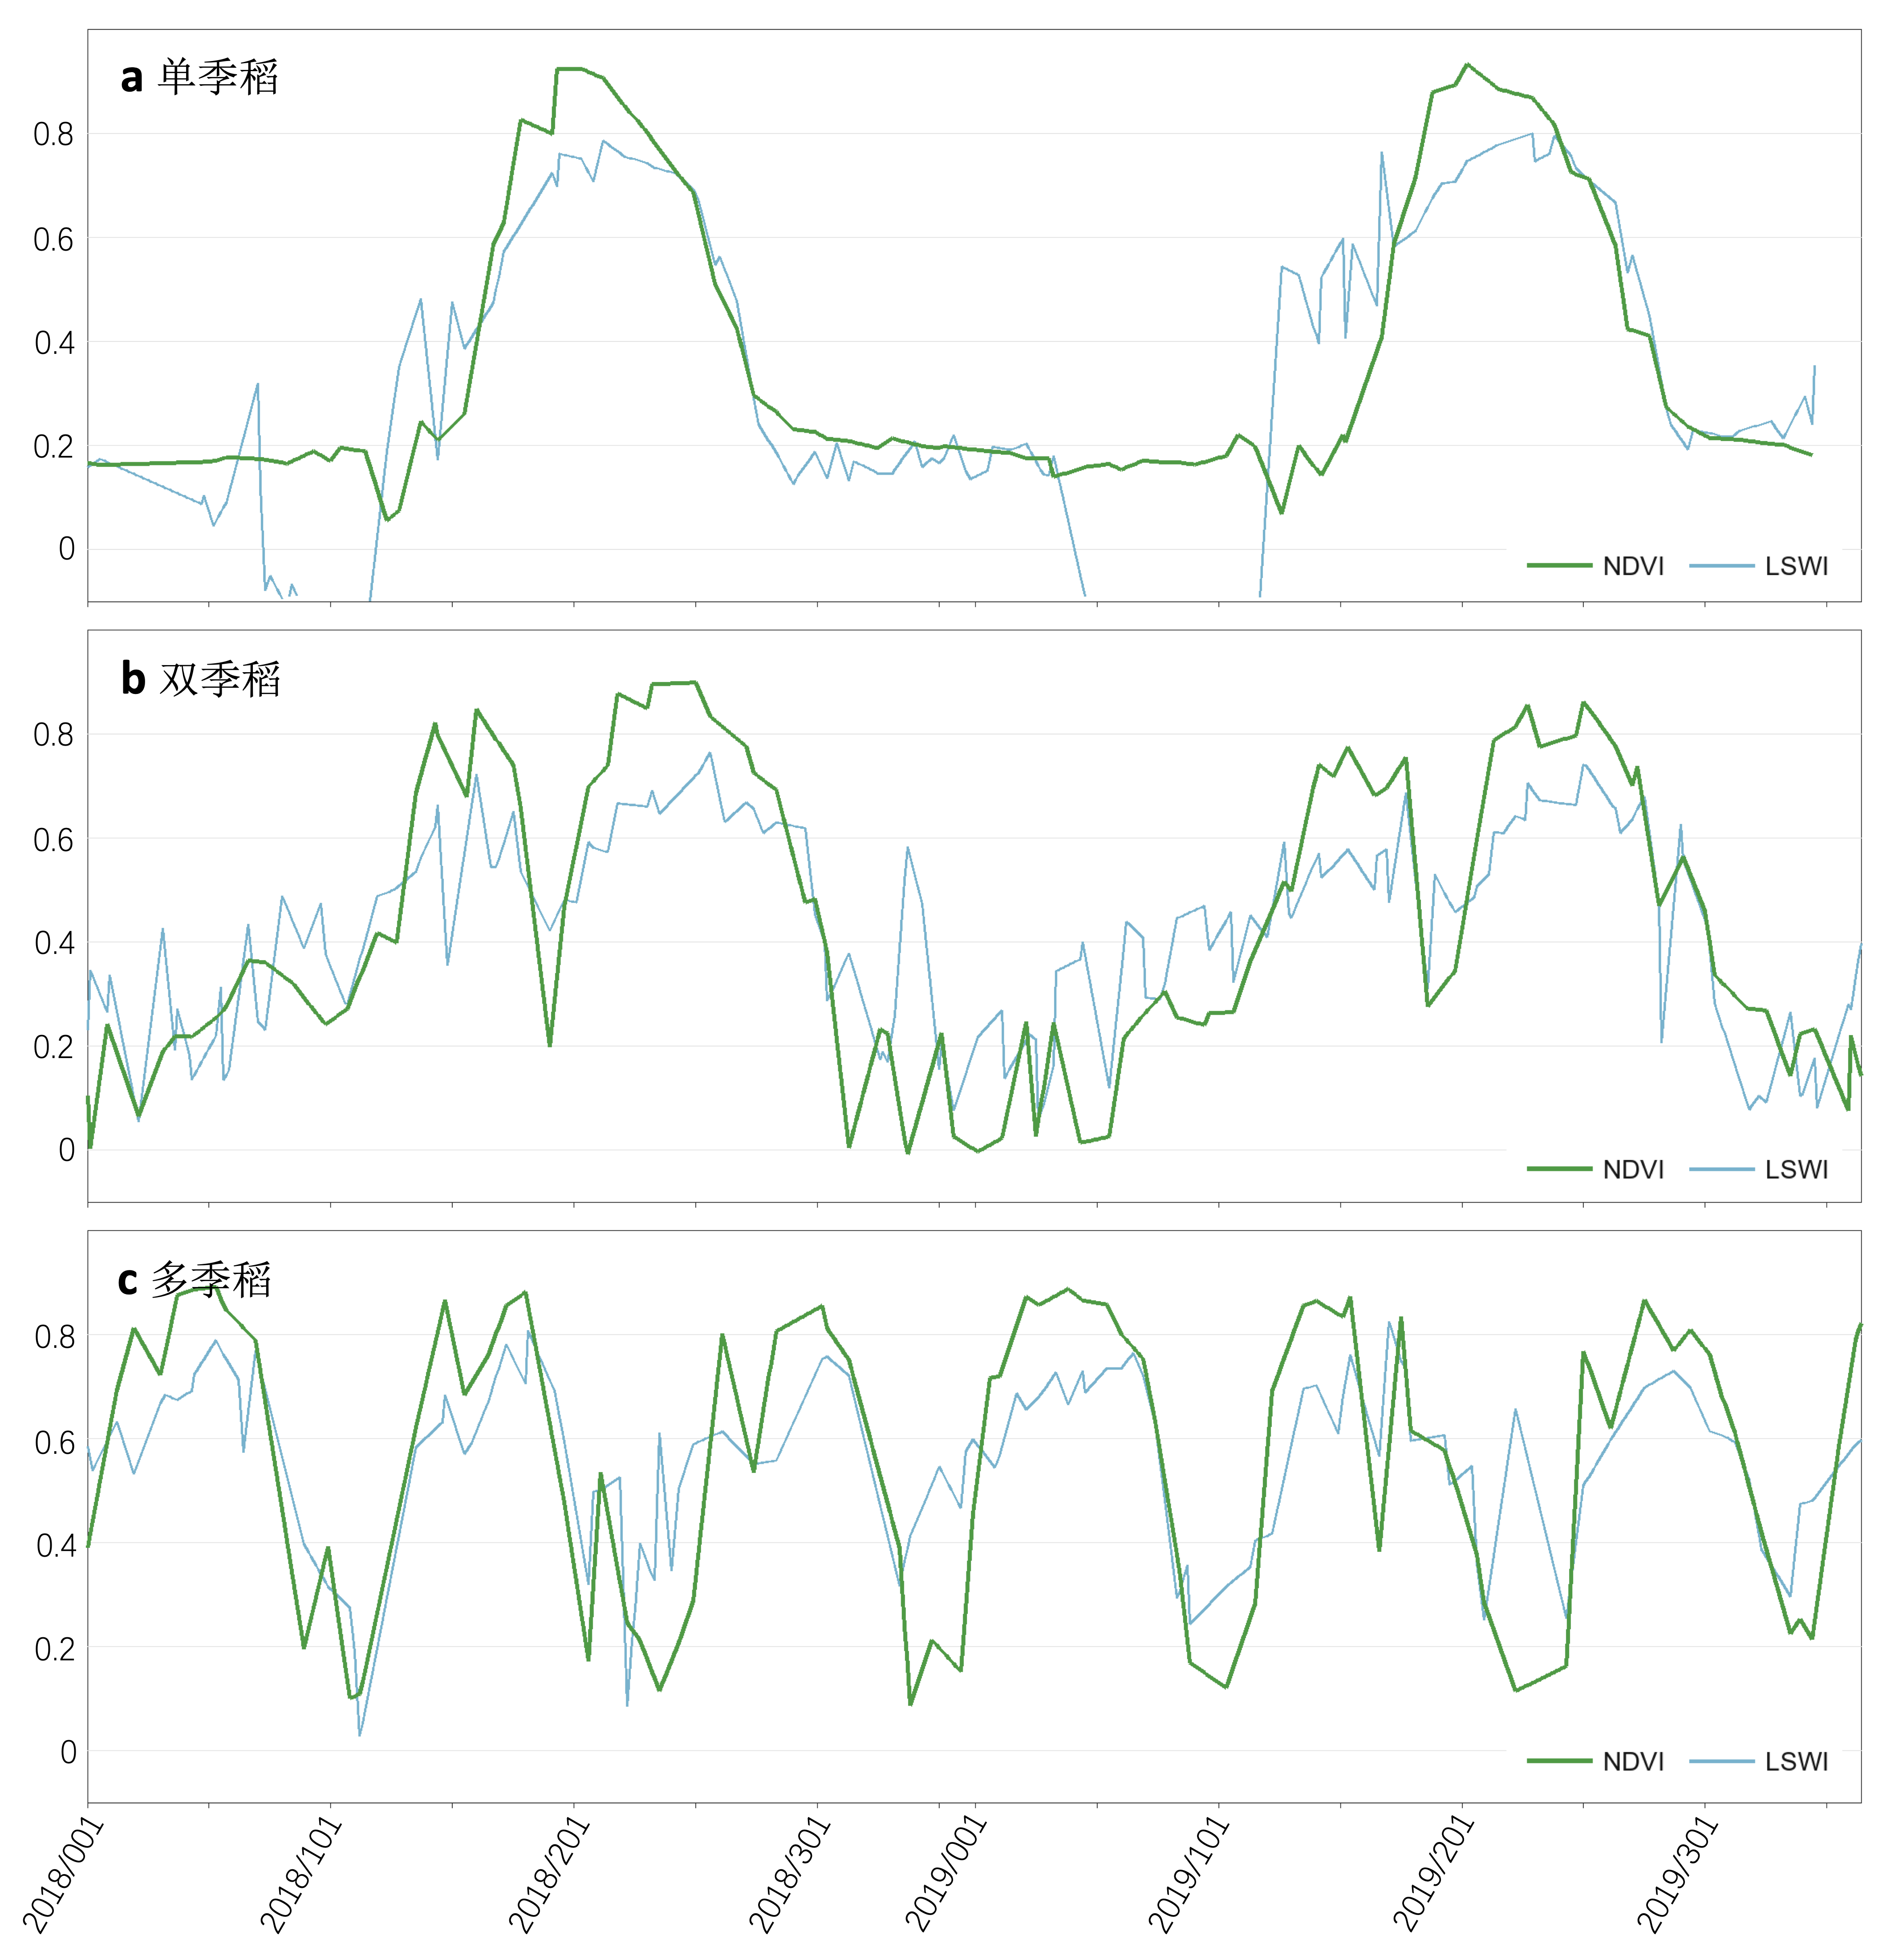
\includegraphics[width=0.95\linewidth]{figure/chapter3/rice_seasons.png}
    \bicaption[不同种植制度下典型水稻像元的 NDVI 和 LSWI 时间序列]{不同种植制度下典型水稻像元的 NDVI 和 LSWI 时间序列：（a）中国东北单季稻样本（45.6937°N，122.9999°E）；（b）中国南方双季稻样本（28.6854°N，112.6057°E）；（c）越南湄公河三角洲三季稻样本（10.3896°N，105.1469°E）。}[Temporal profile of NDVI and LSWI from three typical paddy rice sites with different cropping systems]{Temporal profile of NDVI and LSWI from three typical paddy rice sites with different cropping systems: (a) single paddy rice in Northeast China (45.6937° N, 122.9999° E), (b) double paddy rice in southern China (28.6854° N, 112.6057° E), and (c) triple paddy rice in the Mekong Delta, Vietnam (10.3896° N, 105.1469° E).}
    \label{fig:rice_seasons}
\end{figure}

% 定义研究对象：水稻生长季节
因此，本文将全球水稻动态提取定义为连续日尺度遥感时间序列中的生长季事件识别问题，其核心任务是从像元级 NDVI--LSWI 时间序列中确定水稻生长季的起始、结束及年内发生次数。设像元 \(p\) 具有日尺度 NDVI 序列 \(N_p(t)\) 和 LSWI 序列 \(W_p(t)\)，其识别结果不是单一年度标签，而是一组具有明确时间边界的生长季事件：
\begin{equation}
    \mathcal{E}_p = \{(s_k, e_k)\mid k=1,2,\ldots,n_p\},
    \label{eq:rice_event_set}
\end{equation}
其中，\(s_k\) 和 \(e_k\) 分别表示第 \(k\) 个水稻生长季事件的起始时间（Start of Season, SOS）和结束时间（End of Season, EOS），\(n_p\) 为该像元在给定时间范围内识别出的水稻生长季次数。与年度水稻/非水稻标签相比，式\ref{eq:rice_event_set}直接刻画了同一像元在连续时间轴上的水稻种植过程，使单季、双季、多季以及跨年生长季均可被统一表达。基于水稻生长季的事件集合 \(\mathcal{E}_p\)，年度水稻种植面积、收获面积、复种次数、生长季长度、逐日水稻状态以及环境效应分析所需的真实生长季窗口，均可由像元级生长季事件进一步汇总得到。由此，水稻制图从空间维度上的静态分类转变为时间维度上的事件检测。

% 全球水稻动态提取的算法需求
全球水稻种植制度的高度异质性决定了算法必须具备物候自适应能力。全球水稻播栽期、收获期和种植季次数具有显著区域差异，热带地区水热条件充足，水稻可在全年多个时段播栽，而温带稻区多集中于相对稳定的夏季生长季\cite{Laborte2017SciData,Mishra2021IJAEO}。与此同时，直播、移栽、连续淹水、间歇灌溉、雨养水稻、轮作、休耕和收获后管理等农业实践会改变水稻早期水分信号、植被增长曲线和季间休闲特征，使水稻遥感时序不仅具有自然物候差异，也具有强烈的人为管理差异\cite{Begue2018RS}。如果在全球尺度使用固定月份窗口，南半球稻作可能与北半球窗口错位，热带多季稻可能被遗漏或合并，跨年生长季也可能被自然年边界截断。如果采用固定长度曲线匹配，短季稻会被迫引入无效观测，长季稻则可能丢失关键生育阶段信息。相反，若完全取消物候先验，仅依赖全年曲线匹配，则湿地、水生植被、季节性积水耕地和其他轮作作物可能因局部形态相似而产生较高混淆。

面向上述问题，全球水稻动态提取方法至少需要同时满足三个条件。首先，算法应能够在时间轴上动态搜索候选生长季窗口，即识别候选 SOS 和 EOS，而非完全依赖区域固定播栽月份，以保证热带多熟区、南半球稻区和作物历资料不足区域仍可被识别。其次，候选生长季窗口应依据实际 NDVI--LSWI 曲线变化和本地生长季长度约束自适应确定，而不是按统一天数截断，以避免将不同品种、制度和气候区的水稻强行映射到同一时间尺度。再次，算法应能够判断候选生长季窗口内的曲线是否真正对应水稻生长过程，并根据判定结果决定下一轮搜索起点，从而在同一像元内支持单季、双季、多季和跨年水稻生长季的连续识别。上述要求将水稻物候先验、曲线形态判别和时序反馈机制统一到动态水稻生长季事件识别框架中，使方法既具有可解释的农业遥感机理，又具备全球推广所需的时间弹性。

基于上述条件，本研究设计并开发了水稻生长季事件识别框架 MPD\_DTW（图\ref{fig:mpd_dtw}）。该框架由移动物候检测（Moving Phenological Detection, MPD）模块、动态时间规整（Dynamic Time Warping, DTW）模块和二者之间的反馈机制组成。MPD 模块负责从逐日 NDVI--LSWI 时间序列中搜索候选 SOS 和 EOS，DTW 模块负责比较候选生长季内的 NDVI 曲线与区域标准水稻曲线之间的形态相似性，反馈机制则根据 DTW 判定结果更新下一轮 SOS 搜索起点。由此，MPD 解决“从哪里截取候选曲线”的问题，DTW 解决“截取曲线是否符合水稻生长过程”的问题，反馈机制解决“如何在同一时间轴上连续识别多个季节”的问题。

\begin{figure}[htbp]
    \centering
    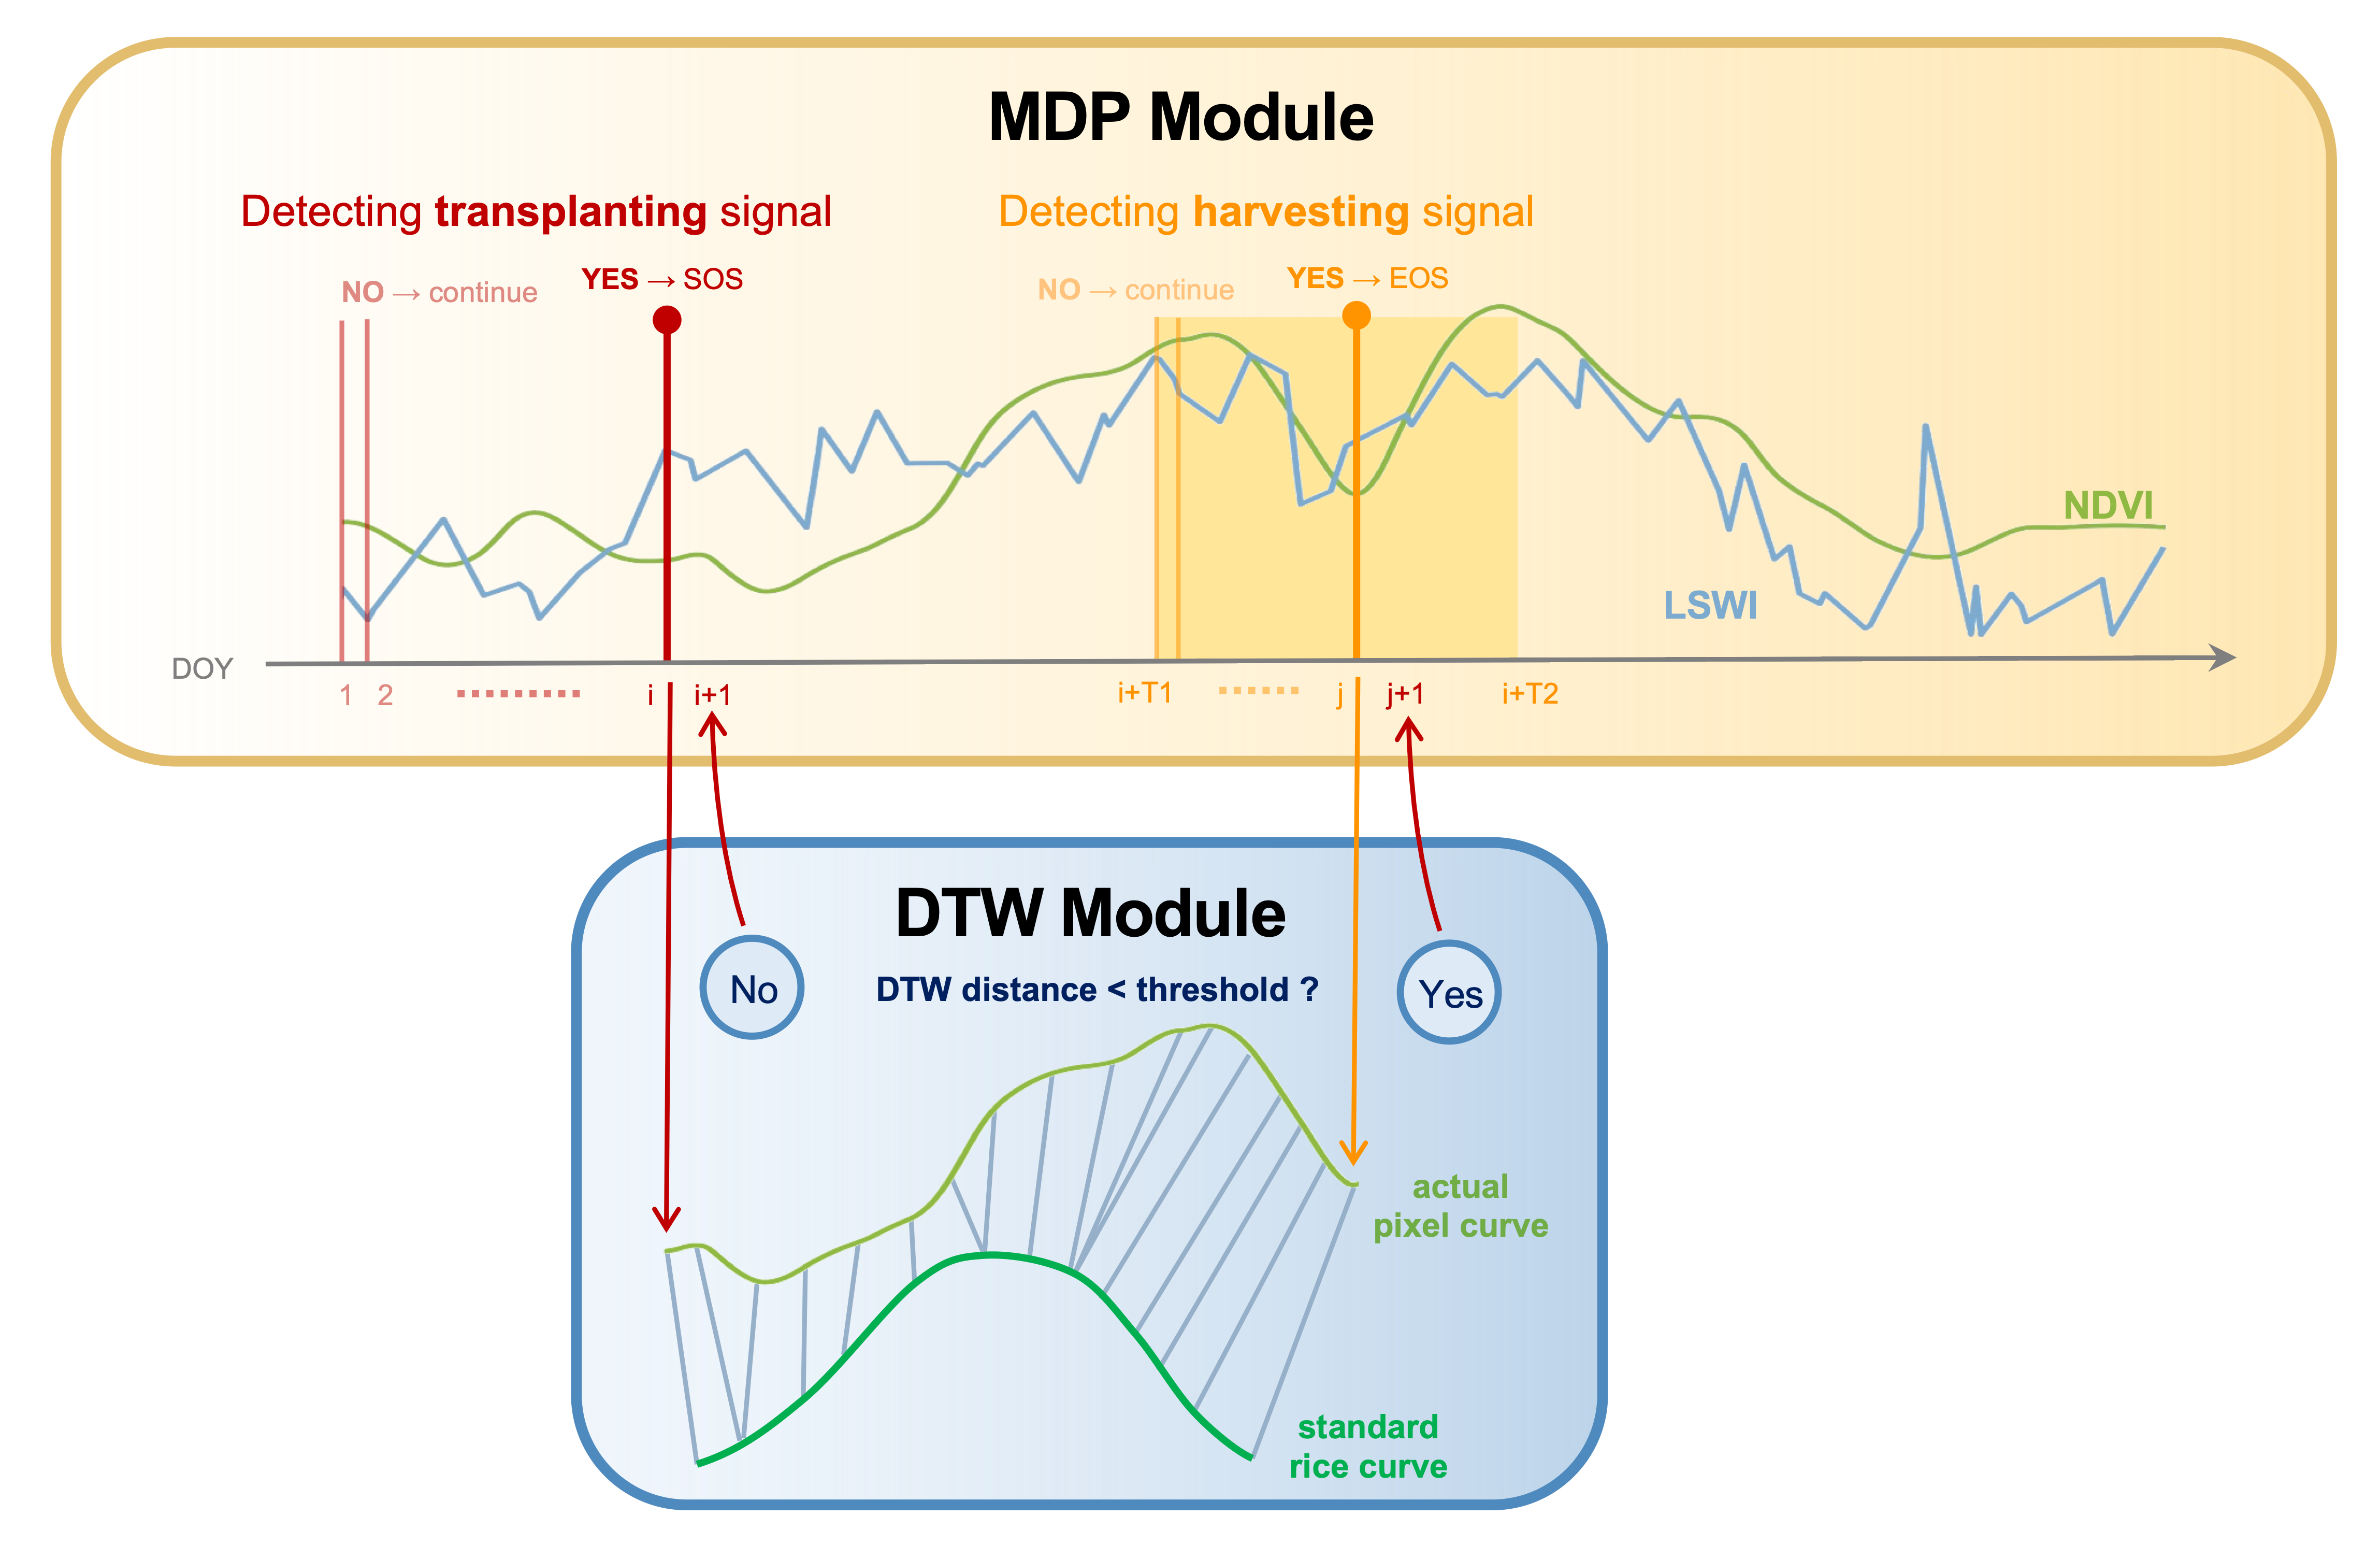
\includegraphics[width=0.99\textwidth]{figure/chapter3/mpd_dtw.png}
    \bicaption{MPD\_DTW 示意图}{Schematic diagram of MPD\_DTW}
    \label{fig:mpd_dtw}
\end{figure}

该设计将物候阈值和曲线匹配置于一个闭环搜索框架中。物候检测为曲线匹配提供具有农业意义的候选边界，避免 DTW 在全年复杂曲线中盲目搜索；曲线匹配检验物候候选是否具有完整水稻生长过程，避免单一淹水信号或局部 NDVI 下降造成误判；反馈机制进一步将单次候选判别转化为连续时间轴上的事件序列识别，使算法能够在同一像元内识别多个非重叠生长季。该框架因而兼具基于物候规则方法的可解释性和基于时间序列相似性方法的弹性，是后续构建全球水稻时空动态数据、分析全球水稻面积变化以及开展真实水稻生长季约束下稻田地表温度效应评估的核心方法基础。

在此基础上，本章研究进一步将 MPD\_DTW 应用于全球尺度长时间序列遥感数据，构建全球水稻时空动态数据集 GlobalRice500。与仅提供年度水稻分布的静态产品不同，GlobalRice500 的基本表达单元是像元级水稻生长季事件。每一次水稻种植均由明确的 SOS 和 EOS 表示，并可进一步汇总为年度水稻种植面积、收获面积、复种次数、生长季长度和逐日水稻状态等变量。由此，GlobalRice500 不仅能够提供全球水稻空间分布信息，也能够刻画水稻种植过程在年内和年际尺度上的动态变化，为全球水稻面积监测、水稻时空格局分析和后续稻田地表温度效应评估提供统一的时空基准。

因此，本章的研究内容包括三个相互衔接的层次：首先，提出基于生长季事件识别的通用水稻动态提取框架 MPD\_DTW，解决全球复杂稻作制度下水稻生长季起止时间和年内发生次数的识别问题；其次，基于该框架构建 GlobalRice500 数据集，并通过高分辨率水稻图和农业统计资料评估其空间一致性和面积可靠性；最后，利用 GlobalRice500 分析 2001--2022 年全球水稻种植面积、生长季特征和区域格局变化。通过上述设计，本章将水稻遥感制图从年度类别判别推进到连续时间轴上的生长季事件识别，并为第四章真实水稻生长季约束下的稻田地表降温效应评估奠定数据基础。


\section{基于生长季事件识别的通用水稻遥感提取框架MPD\_DTW}

\subsection{基于移动物候检测的候选生长季识别}

\label{sec:mpd}

移动物候检测（Moving Phenological Detection, MPD）模块的主要任务，是在逐日遥感时间序列中识别具有水稻物候可能性的候选生长季事件。本研究所称“移动”本质上是一种由物候知识触发并约束的事件级时间推进机制，指的是以候选 SOS 和 EOS 为时间锚点的物候事件递进搜索过程，而非指固定长度时间窗口在全年序列上的机械滑动。MPD 模块沿日尺度时间轴持续检测水稻移栽或返青信号；当某一日期满足 SOS 条件后，随即在该日期之后的一定时间范围内搜索候选 EOS，并将该 SOS--EOS 片段作为一个候选生长季事件 \(c_i=(s_i,e_i)\) 提交给 DTW 模块进行水稻生长过程判别。根据 DTW 判定结果反馈，得到更新后的搜索起点，开始下一个候选生长季事件 \(c_j=(s_j,e_j)\) 的搜索。图\ref{fig:mpd_flowchart}概括了 MPD 模块从日尺度 NDVI--LSWI 序列中检测候选生长季事件的基本流程。

\begin{figure}[htbp]
    \centering
    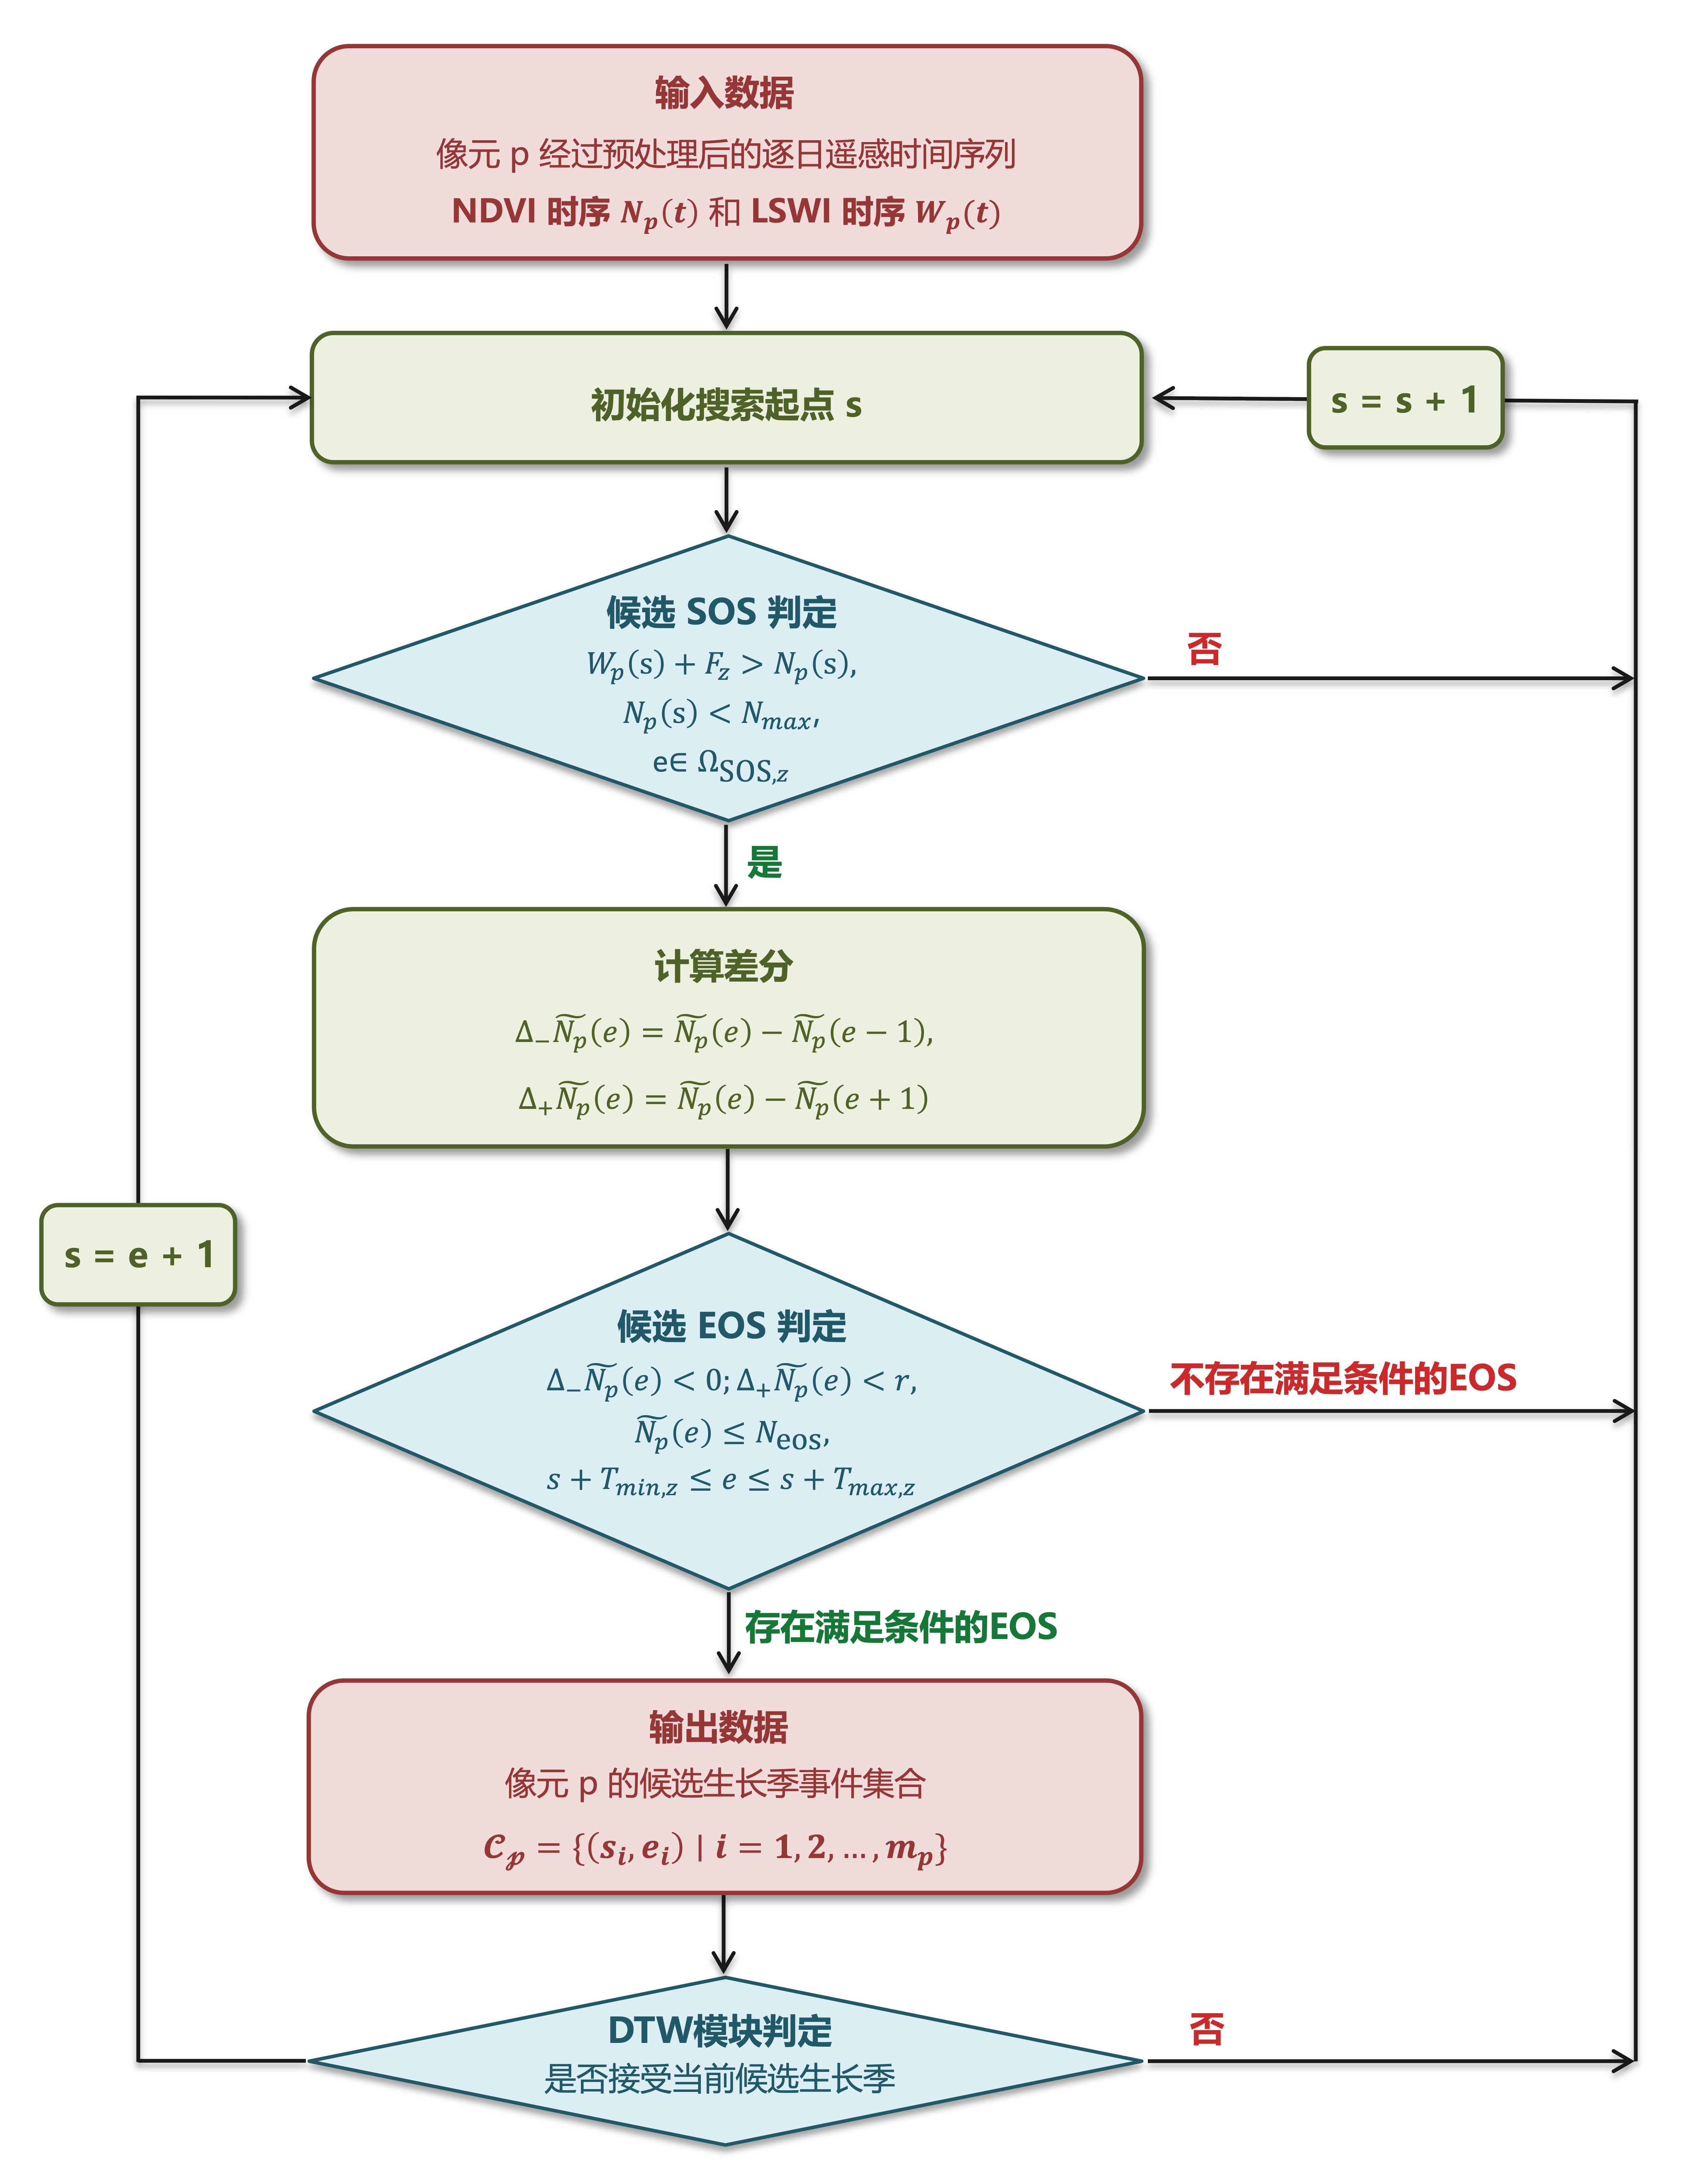
\includegraphics[width=0.95\textwidth]{figure/chapter3/mpd_flowchart.png}
    \bicaption[MPD 模块候选水稻生长季事件检测流程]{MPD 模块候选水稻生长季事件检测流程。MPD 模块以像元级逐日 NDVI--LSWI 时间序列为输入，首先基于水分--植被相对关系识别候选 SOS，随后在合理生长季长度范围内依据 NDVI 衰退特征搜索候选 EOS，并将候选 SOS--EOS 片段提交 DTW 模块进行曲线形态判别；DTW 判定结果进一步反馈更新下一轮搜索起点，从而支持同一像元的单季、双季、多季或跨年水稻生长季的连续识别。}[Workflow of the MPD module for detecting candidate rice growing-season events]{Workflow of the MPD module for detecting candidate rice growing-season events. The MPD module takes pixel-level daily NDVI--LSWI time series as input, identifies candidate SOS based on the relative water--vegetation signal, searches candidate EOS within a plausible growing-season length range according to NDVI decline characteristics, and submits the candidate SOS--EOS segments to the DTW module for curve-shape discrimination. The DTW decision is then used to update the starting point of the next search, enabling continuous identification of single-, double-, multiple-, and cross-year rice growing seasons within the same pixel.}
    \label{fig:mpd_flowchart}
\end{figure}

% 输入数据介绍
MPD\_DTW 的基础输入为像元 \(p\) 的日尺度 NDVI 序列和 LSWI 序列。本文以 \(N_p(t)\) 和 \(W_p(t)\) 分别表示像元 \(p\) 在日期 \(t\) 的 NDVI 和 LSWI，其中 \(t\) 为以年积日（Day of Year, DOY）表示的日尺度时间索引；二者均由第\ref{sec:vi_preprocess}节所述预处理流程获得。NDVI 和 LSWI 在 MPD 判定中承担不同的物候识别功能。NDVI 主要用于刻画完整作物生长季曲线及其局部变化，因此在进入物候检测前，本文采用 41 d 窗口、3 阶多项式的 Savitzky--Golay 滤波对日尺度 NDVI 序列进行平滑，以降低残余云、气溶胶、双向反射差异和异常低值对曲线形态及局部导数判断的影响。Savitzky--Golay 滤波通过局部多项式拟合，在抑制高频噪声的同时尽量保留曲线峰值宽度和线型特征，已被广泛应用于植被指数时间序列重建\cite{Chen2004RSE}。设像元 \(p\) 的原始日尺度 NDVI 序列为 \(N_p(t)\)，平滑后的 NDVI 表示为：
\begin{equation}
    \widetilde{N}_p(t)=\mathrm{SG}_{41,3}\{N_p(t)\}.
    \label{eq:sg_ndvi}
\end{equation}
LSWI 更侧重捕捉水稻移栽或返青初期浅水层、湿润土壤和稀疏植被共同作用形成的短时水分信号。为避免过度平滑削弱淹水信号的时间位置和相对幅度，LSWI 在获得日尺度序列后不再进行额外的平滑处理，直接用于刻画水分背景的时序变化。

% SOS 的淹水物候依据
水稻区别于多数旱地作物的关键遥感特征，来自移栽或返青初期浅水层、湿润土壤和稀疏幼苗共同作用形成的水分--植被组合信号。短波红外波段对地表和冠层液态水高度敏感，因此基于近红外和短波红外波段构建的 LSWI 能够表征植被与土壤背景水分变化\cite{Gao1996}。在典型移栽稻田中，早期浅水覆盖增强 LSWI，而绿色植被覆盖度仍较低，NDVI 尚未进入快速上升阶段；随着水稻返青、分蘖和冠层闭合，NDVI 迅速升高并逐渐超过水分信号。基于上述物候机理，MPD 模块的候选 SOS 由日尺度 NDVI 与 LSWI 的相对关系触发。移栽或返青初期稻田浅水层和湿润土壤会增强短波红外相关水分信号，使 LSWI 接近或高于 NDVI/EVI，从而形成区别于多数旱作物的水分--植被组合特征\cite{Xiao2005,Xiao2006}。

然而，一个像元可能并非完全由稻田组成，稻田、田埂、沟渠、裸土和其他作物常共同组成混合像元，水稻淹水信号可能被亚像元异质性削弱，这也是中低分辨率水稻制图误差的重要来源\cite{Teluguntla2015RS,Han2021}。在 Cui 等基于多时相 Landsat 的水稻制图研究中，\(\mathrm{LSWI}+0.05>\mathrm{NDVI}\)被用于识别移栽阶段淹水的水稻像元\cite{Cui2015}，说明在水分指数与植被指数比较中引入适度容忍项具有明确的遥感物候依据。因此，为增强候选 SOS 生成对混合像元、弱淹水稻田和不同水分管理方式的适应性，本文在 LSWI 与 NDVI 的相对判据中引入的洪水因子 \(F_z\)，将其作为水分信号判定的容忍项。对像元 \(p\) 在日期 \(t\) 的候选 SOS 判定为：
\begin{equation}
    W_p(t)+F_z>\widetilde{N}_p(t), \quad
\widetilde{N}_p(t)<N_{\mathrm{sos}}, \quad
    t\in\Omega_{\mathrm{SOS},z},
    \label{eq:sos_condition}
\end{equation}
其中，\(F_z\) 为参数区 \(z\) 的洪水因子，\(N_{\mathrm{sos}}=0.5\) 为起始期 NDVI 上限，\(\Omega_{\mathrm{SOS},z}\) 为该参数区允许搜索的候选 SOS 日期集合。

\(F_z\) 的本质是对混合像元条件下弱化淹水信号的一种补偿机制：当 \(F_z=0\) 时，只有 LSWI 接近或高于 NDVI 的强水分信号能够触发 SOS；当 \(F_z>0\) 时，部分因像元混合、稻田破碎化、间歇灌溉或雨养条件导致 LSWI 略低于 NDVI 的真实水稻候选期仍可被保留。\(F_z\) 仅用于候选事件生成阶段，用于减少因混合像元导致的水稻起始期漏识别；候选 SOS--EOS 片段是否最终被接受为水稻生长季，仍需由后续 DTW 模块基于完整 NDVI 生长过程进行判别。\(N_{\mathrm{sos}}\) 用于排除已经进入高冠层覆盖阶段的日期，避免将旺盛生长期误判为生长季起点。\(\Omega_{\mathrm{SOS},z}\) 表示参数区 \(z\) 中允许触发候选 SOS 的日期集合，用于在候选起始期搜索中剔除明显不符合水稻播栽物候的时段。对于基于 LSWI 与 NDVI 相对关系的淹水信号识别而言，早春积雪消融、短期地表积水或非稻田湿润背景也可能产生类似水稻移栽期的水分响应\cite{Zhang2015ISPRS,Qin2015ISPRS}。

% EOS 的收获物候依据
在候选 SOS 被触发后，MPD 进一步依据水稻成熟收获后的绿度衰退特征搜索候选 EOS。水稻从抽穗灌浆进入成熟阶段后，叶片衰老、含绿量下降；收获后地表由高生物量冠层转为残茬、裸土、浅水或翻耕背景，NDVI 通常出现快速下降并逐渐趋于低值。SOS 判定侧重水分--植被相对关系，EOS 判定则主要依赖 NDVI 曲线的局部衰退特征。
对于每个候选 SOS \(s\)，本研究基于水稻物候学和农业遥感先验知识确定参数区 \(z\) 内水稻生长季持续时间的合理范围，得到候选 EOS 相对于候选 SOS 的时间滞后约束，即 SOS--EOS 时间间隔范围。在该时间间隔范围内，MPD 模块进一步依据 NDVI 衰退特征检测候选 EOS。
\begin{equation}
    s+T_{\min,z}\leq e\leq s+T_{\max,z},
    \label{eq:growing_length}
\end{equation}
其中，\(T_{\min,z}\) 和 \(T_{\max,z}\) 分别表示参数区 \(z\) 中候选 SOS 与候选 EOS 之间时间间隔的下限和上限。该约束的核心作用是保证候选 SOS--EOS 片段具有合理的水稻生育持续时间，避免将明显短于真实生长季的短期积水、云噪声或非作物扰动识别为候选水稻季，同时防止候选片段过长而跨越真实收获期并吞并后续种植季。

在式\ref{eq:growing_length}限定的窗口内，候选 EOS 需同时满足 NDVI 已从前一日下降、当前日之后下降速度减弱或趋稳，且 NDVI 已回落至收获期低值范围。记平滑 NDVI 的前一日差分和后一日差分分别为：
\begin{equation}
    \Delta_{-}\widetilde{N}_p(e)=\widetilde{N}_p(e)-\widetilde{N}_p(e-1),
    \quad
    \Delta_{+}\widetilde{N}_p(e)=\widetilde{N}_p(e)-\widetilde{N}_p(e+1).
    \label{eq:ndvi_derivatives}
\end{equation}
则候选 EOS 的判定条件为：
\begin{equation}
    \Delta_{-}\widetilde{N}_p(e)<0,\quad
    \Delta_{+}\widetilde{N}_p(e)<r,\quad
    \widetilde{N}_p(e)\leq N_{\mathrm{eos}},
    \label{eq:eos_condition}
\end{equation}
其中，\(r=0.0025\) 为成熟期下降后趋稳的速率阈值，\(N_{\mathrm{eos}}=0.5\) 为收获期 NDVI 上限。式\ref{eq:eos_condition}并不要求 EOS 是全年 NDVI 的绝对最小值，而是要求其出现在候选 SOS 之后符合农业遥感先验知识的时间间隔范围内，并表现为由高绿度阶段衰退后的近局部低值。若某一候选 SOS 后不存在满足该条件的 EOS，则该 SOS 不构成完整候选生长季，算法继续向后搜索新的候选 SOS。

% 候选季节集合生成
为区别于经 MPD\_DTW 判别后形成的最终水稻生长季事件集合 \(\mathcal{E}_p\)，本章研究将 MPD 阶段生成但尚未经过 DTW 判别的 SOS--EOS 片段称为候选生长季事件。对于像元 \(p\)，所有候选生长季事件构成候选事件集合：
\begin{equation}
    \mathcal{C}_p = \{(s_i, e_i)\mid i=1,2,\ldots,m_p\},
    \label{eq:candidate_event_set}
\end{equation}
其中，\(s_i\) 和 \(e_i\) 分别表示第 \(i\) 个候选生长季事件的候选 SOS 和候选 EOS，\(m_p\) 为 MPD 阶段在像元 \(p\) 的时间序列中生成的候选事件数量。

对于任一候选 SOS \(s\)，MPD 可能识别出一个或多个满足收获期条件的候选 EOS。本章研究将由同一 SOS 生成的候选生长季片段表示为：令 \(I_{\mathrm{EOS}}(e)\in\{0,1\}\) 为收获期指示函数，当日期 \(e\) 满足式\ref{eq:eos_condition}的 EOS 判据时取值为 1，否则为 0。
\begin{equation}
    \mathcal{C}_p(s)=\{(s,e)\mid e\in\Omega_{\mathrm{EOS}}(s),\ I_{\mathrm{EOS}}(e)=1\},
    \label{eq:candidate_set}
\end{equation}
其中，\(\Omega_{\mathrm{EOS}}(s)\) 为式\ref{eq:growing_length}定义的 EOS 搜索窗口，\(I_{\mathrm{EOS}}(e)=1\) 表示日期 \(e\) 满足式\ref{eq:eos_condition}的收获期判据。MPD 阶段不直接在多个 \(e\) 中确定最终 EOS，而是将候选 SOS--EOS 曲线交由 DTW 模块计算与标准水稻曲线的相似性，并由最小 DTW 距离决定该 SOS 对应的最优 EOS。该处理避免了仅凭局部 NDVI 极小值确定收获期所导致的不稳定性，使 EOS 同时受到收获物候和完整生长曲线形态的约束。

MPD 模块逐日移动识别策略的核心价值在于摆脱固定作物历对全球制图的限制。温带单季稻候选 SOS 往往集中于春末夏初，EOS 集中于秋季；热带和亚热带多季稻可在一年内出现多个候选 SOS；南半球和跨年稻作系统则可能在自然年后部起始、次年完成收获。只要 NDVI--LSWI 时间序列中存在符合淹水或返青、冠层发育、成熟收获的连续过程，MPD 模块即可生成候选生长季。然而，季节性湿地、水生植被、短期积水旱地以及部分轮作作物也可能在局部时段产生类似的水分增强、绿度变化或绿度衰退特征\cite{Zhan2021}。因此，MPD 阶段生成的候选事件仅表明该 SOS--EOS 片段具有水稻物候可能性，其功能定位是为后续曲线匹配提供候选时间边界，而非完成最终水稻判定。候选片段是否构成真实水稻生长季，仍需由 DTW 模块基于完整生长过程的曲线形态进一步判别。

\subsection{基于动态时间规整的水稻生长过程判别}

\label{sec:dtw}

% 总述：DTW模块的作用
在 MPD 模块确定候选 SOS--EOS 边界之后，水稻识别任务由局部物候事件检测转向完整生长过程判别。本章研究基于动态时间规整（Dynamic Time Warping, DTW）模块进行曲线形态检验，度量候选生长季 NDVI 曲线与区域标准水稻生长曲线之间的相似性。与仅依据淹水日、成熟日或峰值大小的局部判据不同，DTW 面向完整生长季曲线，重点检验低值起始、快速增绿、峰值维持和成熟下降等阶段是否按照水稻典型生育顺序连续出现。

% 为何需要分区构建标准曲线：全球种植制度多样
水稻生长过程在遥感植被指数曲线形态上通常具有较强的阶段性。移栽或返青初期，NDVI 往往处于较低水平；随后随着返青、分蘖和冠层快速发育，NDVI 迅速上升；在抽穗和灌浆阶段，冠层绿度维持在较高水平；成熟收获后，NDVI 又随植被覆盖和生物量下降而回落。这种相对稳定的阶段序列，使基于时间序列形态的水稻识别具有明确的物候基础。

在全球尺度上，上述阶段序列并不会以固定长度或固定日期出现。不同稻作制度、气候背景和管理方式会显著改变水稻生长季长度和物候相位：热带短季稻可能在约三个月内完成一个生长季，温带单季稻可持续五个月以上，双季稻和三季稻中每一季的长度又常短于单季稻\cite{Laborte2017SciData,Mishra2021IJAEO}。为应对这种区域性和制度性物候差异，本章研究未采用单一全球标准曲线，而是根据主要稻区的物候特征分别构建区域化标准水稻曲线，使不同气候背景和种植制度下的典型生长节律能够在 DTW 判别中得到合理表征。

% 为何需要DTW（非线性匹配）：相同种植制度仍有细微差异
区域化标准水稻曲线能够表征不同稻区和不同种植制度下的典型生长节律，但其本质上仍是参数区内水稻生长过程的代表性模板，难以完全覆盖同一参数区或同一种植制度内部的物候变异。即使同为单季稻，不同品种、生育期类型、播栽日期、积温条件、水分管理和年际气候波动仍可能改变水稻各生育阶段在时间轴上的位置，导致返青、峰值和成熟阶段相对于标准曲线发生提前、滞后或局部拉伸。对于这种情况，候选曲线与标准曲线之间的差异并不一定意味着二者生长过程不同，也可能仅反映同一水稻生长过程在时间尺度上的伸缩和相位偏移。

这种内部的物候相位偏移和生长速率差异，使固定时间轴曲线相似性度量难以稳定适用于全球水稻制图。第~\ref{sec:curve_similarity_methods}~节所述的欧氏距离、均方误差、相关系数或光谱角等方法，通常将待分类曲线与标准曲线视为定义在同一时间轴上的向量，并隐含相同序列位置大体对应相同生育阶段的假设。该假设在播栽期集中、生长季窗口稳定的区域可以近似成立，但在全球尺度和复杂稻作制度下往往难以满足。当候选曲线与标准曲线具有相似的水稻生长形态、但关键阶段出现时间不一致时，固定时间轴度量容易将物候相位差异误判为曲线形态差异。若通过截断、填充或重采样强制统一曲线长度，又可能引入非生长季或低质量观测，削弱返青、旺盛生长和成熟下降等关键阶段的形态信息。因此，本文需要采用能够在保持生育阶段顺序的同时允许局部时间弹性的曲线匹配方法。

动态时间规整（Dynamic Time Warping, DTW）通过允许局部时间轴发生非线性拉伸或压缩，为候选曲线与标准水稻曲线之间的阶段对齐提供了时间弹性\cite{Petitjean2012}，被广泛用于遥感时间序列的物候匹配、土地覆盖制图和作物类型识别\cite{Maus2016,Belgiu2018}。在这种非线性匹配机制下，候选曲线中的返青、旺盛生长和成熟下降等关键生育阶段能够与标准曲线中的相同阶段相互对应，而不要求它们发生在完全相同的序列位置。换言之，DTW 比较的是候选 SOS--EOS 片段内部的阶段顺序和整体形态，而不是固定日期上的逐点相似性。图\ref{fig:dtw_schematic}展示了 DTW 非线性时间轴弯曲和最优路径匹配的基本原理。

\begin{figure}[htbp]
    \centering
    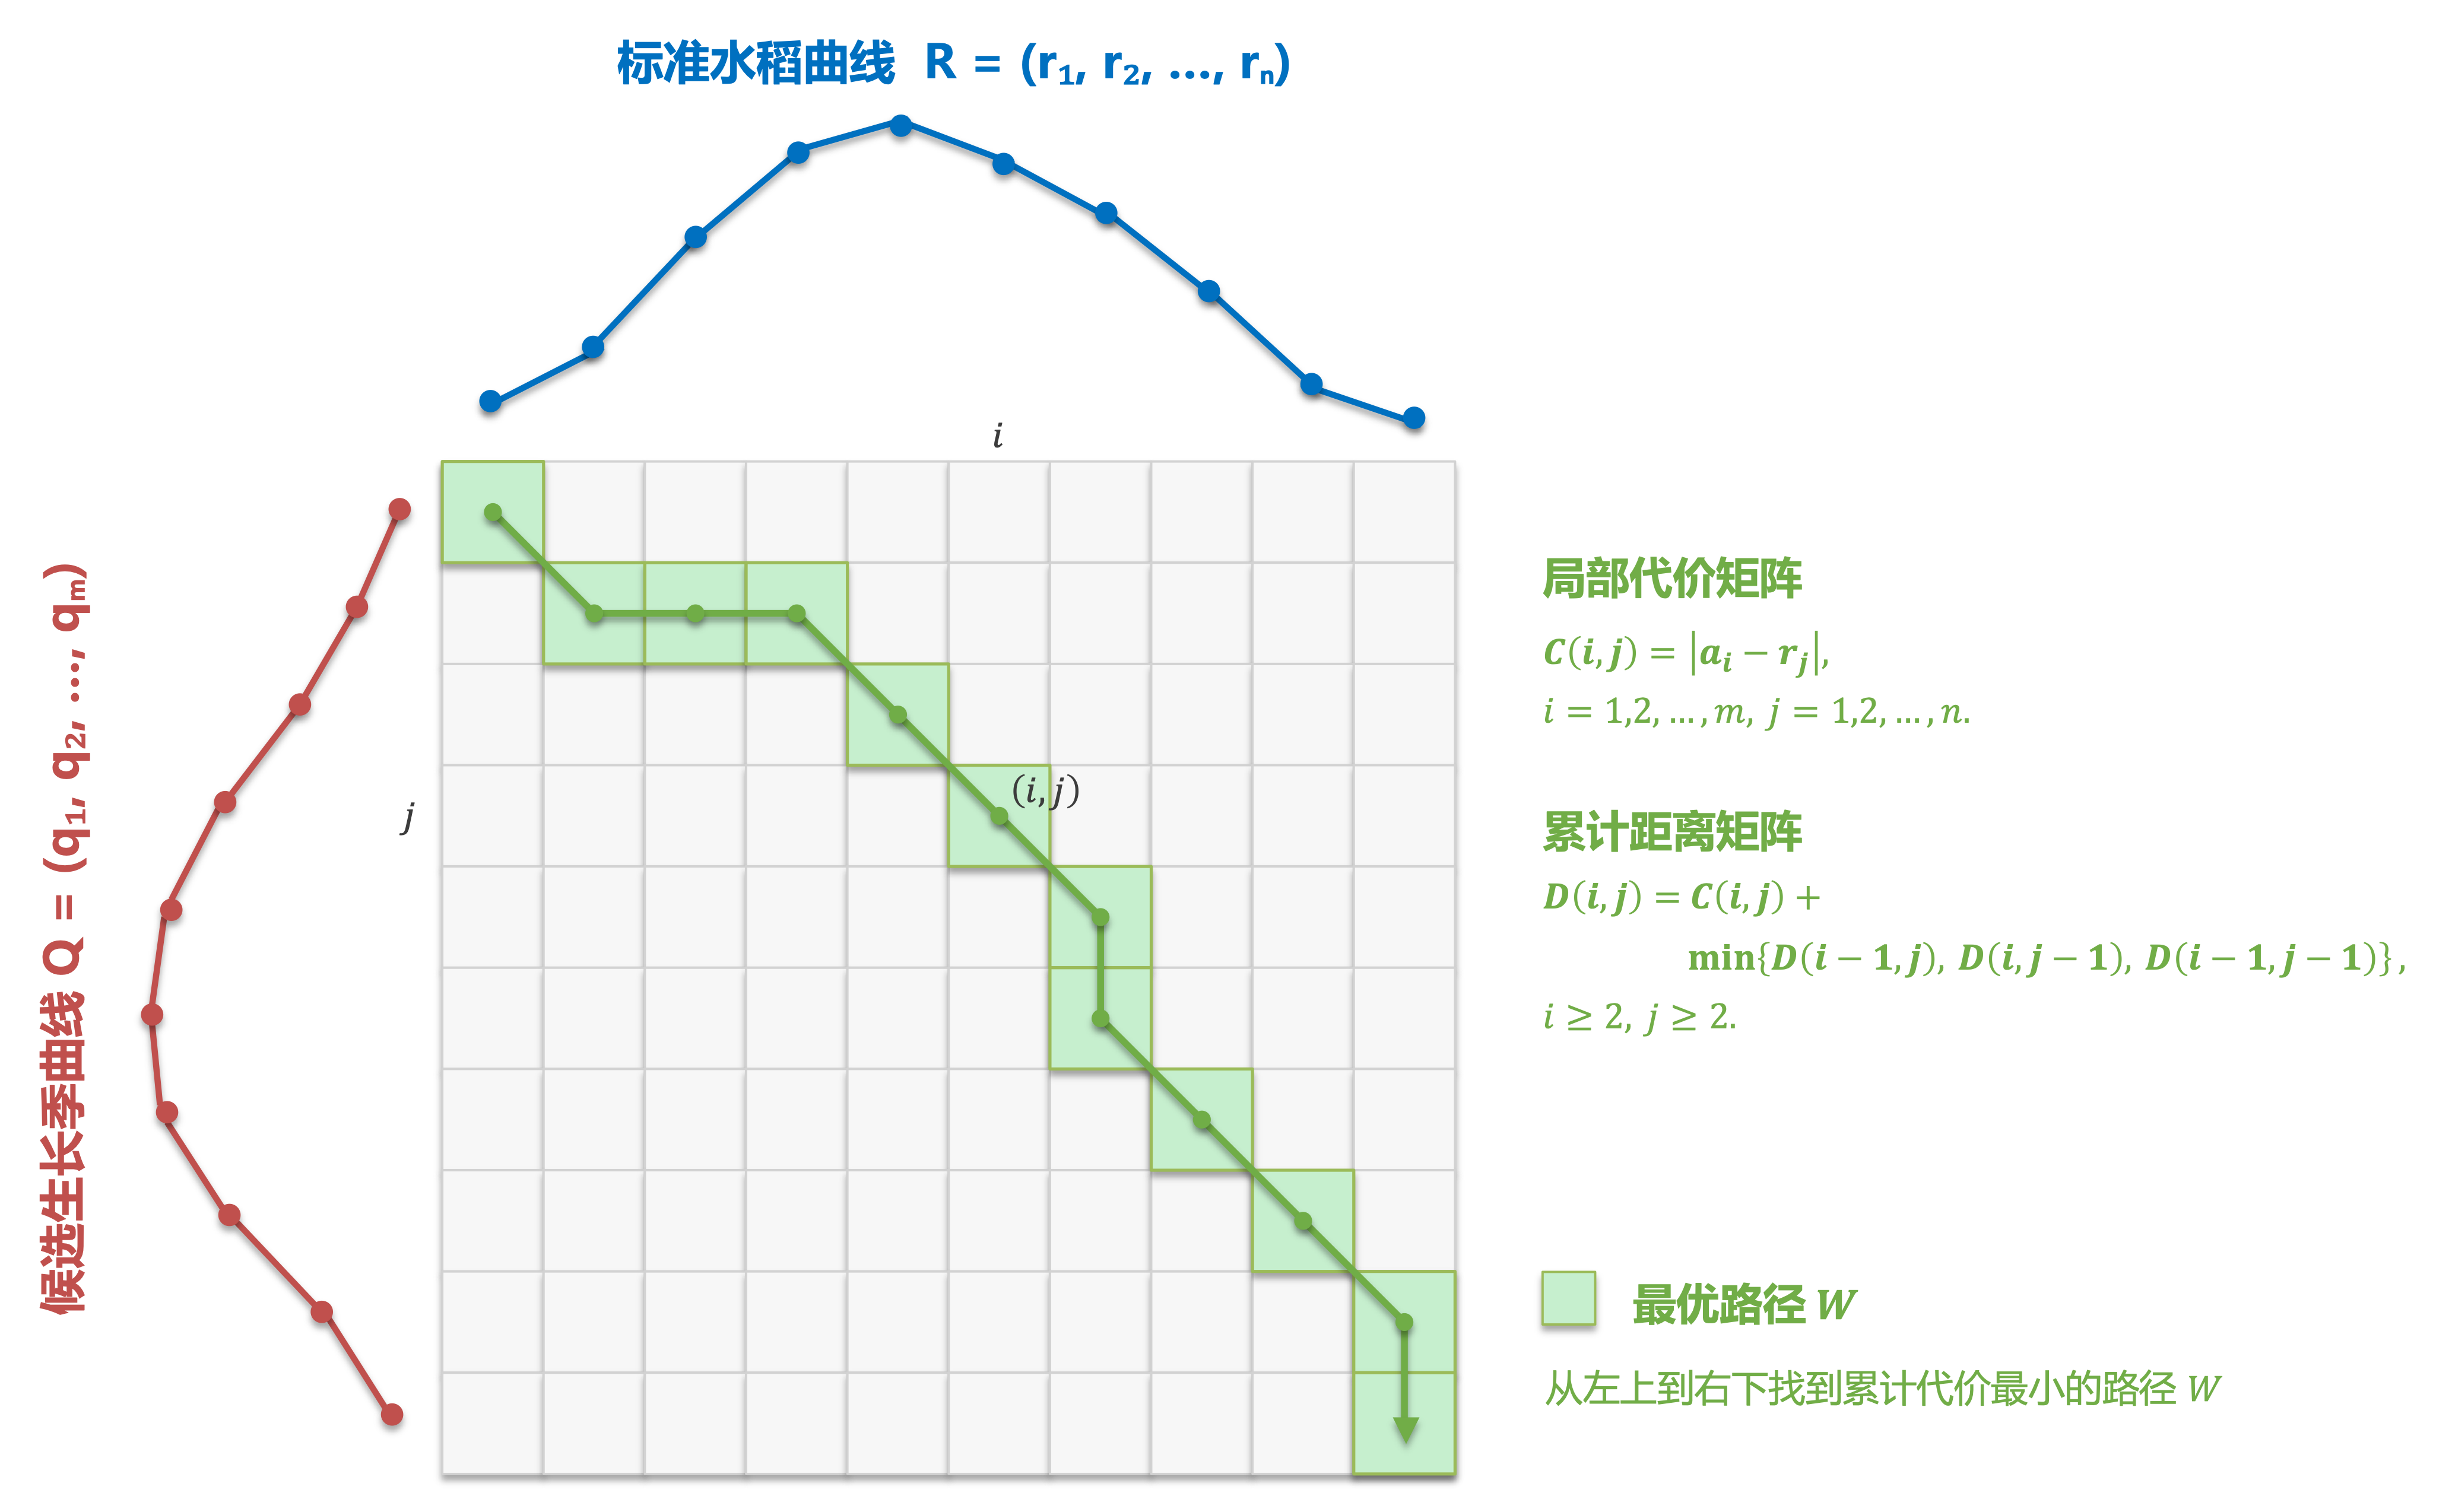
\includegraphics[width=0.95\textwidth]{figure/chapter3/dtw_schematic.png}
    \bicaption{DTW 用于候选生长季曲线与标准水稻曲线非线性匹配的原理示意图}{Schematic diagram of nonlinear curve matching between a candidate growing-season curve and a standard rice curve using DTW}
    \label{fig:dtw_schematic}
\end{figure}

% DTW 基本原理与数学定义
DTW 是一种经典的动态规划时间序列匹配方法，能够在保持时间顺序约束的同时寻找两条序列之间的最优匹配路径\cite{Sakoe1978}。设候选生长季 NDVI 曲线为 \(A=(a_1,a_2,\ldots,a_m)\)，标准水稻曲线为 \(R=(r_1,r_2,\ldots,r_n)\)，其中 \(m\) 与 \(n\) 分别为两条序列的长度。DTW 旨在保持时序单调性约束的前提下，寻找两条序列之间的最优时间对应关系，使总体匹配代价最小。

首先，构造局部代价矩阵（local cost matrix）\(\mathbf{C}\in\mathbb{R}^{m\times n}\)，即图\ref{fig:dtw_schematic}中的灰色网格。局部代价矩阵的元素表示候选曲线与标准曲线在对应时间点上的局部差异。本研究采用绝对距离度量局部代价：
\begin{equation}
    C(i,j)=|a_i-r_j|,\quad i=1,2,\ldots,m,\ j=1,2,\ldots,n.
    \label{eq:dtw_local_cost}
\end{equation}

DTW 通过动态规划寻找一条从 \((1,1)\) 到 \((m,n)\) 的最优规整路径（warping path）\(W=(w_1,w_2,\ldots,w_K)\)，其中 \(w_k=(i_k,j_k)\) 表示候选曲线第 \(i_k\) 个元素与标准曲线第 \(j_k\) 个元素之间的对应关系。该路径需满足边界条件、单调性和连续性三类约束。

边界条件要求路径必须从两条序列的起点开始并在终点结束：
\begin{equation}
    w_1=(1,1),\quad w_K=(m,n).
    \label{eq:dtw_boundary}
\end{equation}

单调性要求路径在时间轴上不可逆：
\begin{equation}
    i_k\le i_{k+1},\quad j_k\le j_{k+1},\quad \forall k=1,2,\ldots,K-1.
    \label{eq:dtw_monotonicity}
\end{equation}

连续性要求路径每次只能向前推进一个时间步，且不允许原地停留：
\begin{equation}
    i_{k+1}-i_k\in\{0,1\},\quad j_{k+1}-j_k\in\{0,1\},\quad (i_{k+1}-i_k)+(j_{k+1}-j_k)\ge 1.
    \label{eq:dtw_continuity}
\end{equation}

在上述约束下，路径 \(W\) 的累计代价定义为路径上所有局部代价之和：
\begin{equation}
    \mathcal{C}(W)=\sum_{k=1}^{K}C(i_k,j_k).
    \label{eq:dtw_path_cost}
\end{equation}

通过构建累计距离矩阵（cumulative distance matrix）\(\mathbf{D}\in\mathbb{R}^{m\times n}\)，DTW 可以求解两条曲线之间的最优匹配路径，即图\ref{fig:dtw_schematic}中的绿色路径。累计距离矩阵元素的递推定义如下：

边界初始化：
\begin{equation}
    D(1,1)=C(1,1),
    \label{eq:dtw_init}
\end{equation}
\begin{equation}
    D(i,1)=D(i-1,1)+C(i,1),\quad i=2,3,\ldots,m,
    \label{eq:dtw_init_i}
\end{equation}
\begin{equation}
    D(1,j)=D(1,j-1)+C(1,j),\quad j=2,3,\ldots,n.
    \label{eq:dtw_init_j}
\end{equation}

内部递推关系为：
\begin{equation}
    D(i,j)=C(i,j)+\min\bigl\{D(i-1,j),\,D(i,j-1),\,D(i-1,j-1)\bigr\},\quad i\ge 2,\ j\ge 2.
    \label{eq:dtw_recurrence}
\end{equation}

递推式中的三种转移方向分别对应候选曲线时间轴拉伸、标准曲线时间轴拉伸以及两条曲线同步推进。该三邻域递推形式与常用的对称步进模式 symmetric1 一致，能够在允许局部时间弹性的同时保持两条序列的整体时序结构\cite{Sakoe1978,Petitjean2012}。最终，两条序列之间的 DTW 距离定义为最优路径的累计代价，即累计距离矩阵的右下角元素：
\begin{equation}
    \mathrm{DTW}(A,R)=D(m,n).
    \label{eq:dtw_distance}
\end{equation}

最优规整路径可通过从 \((m,n)\) 逆向回溯至 \((1,1)\) 得到。在每一步 \((i,j)\) 处，选择使累计距离最小的前驱节点：
\begin{equation}
    (i_{k-1},j_{k-1})=\arg\min_{(i',j')\in\mathcal{N}(i,j)}D(i',j'),
    \label{eq:dtw_backtrack}
\end{equation}
其中 \(\mathcal{N}(i,j)=\{(i-1,j-1),(i-1,j),(i,j-1)\}\) 为当前节点的有效前驱集合。该回溯过程刻画了候选曲线与标准曲线之间的非线性时间对应关系，使不同生育阶段能够在时间轴上弹性对齐。

% 曲线相似性度量与水稻判定
设 MPD 模块生成的候选生长季 NDVI 曲线为 \(A_{s:e}=(a_1,a_2,\ldots,a_m)\)，其中 \(s\) 和 \(e\) 分别表示候选 SOS 和候选 EOS；
参数区 \(z\) 的标准水稻曲线记为 \(R_z=(r_1,r_2,\ldots,r_n)\)。
对于任一候选曲线 \(A_{s:e}\) 与标准曲线 \(R_z\)，
按照式\ref{eq:dtw_local_cost}--\ref{eq:dtw_distance}构建局部代价矩阵和累计距离矩阵，并通过动态规划获得二者之间的 DTW 距离：
\[
    d_z(s,e)=\mathrm{DTW}(A_{s:e},R_z).
\]

% 设 MPD 模块生成的候选生长季 NDVI 曲线为 \(A_{s:e}=(a_1,a_2,\ldots,a_m)\)，其中 \(s\) 和 \(e\) 分别表示候选 SOS 和候选 EOS；参数区 \(z\) 内的标准水稻曲线集合记为 \(\mathcal{R}_{z}=\{R_q\}\)，其中 \(R_q=(r_1,r_2,\ldots,r_n)\)。对于任一候选曲线 \(A_{s:e}\) 与标准曲线 \(R_q\)，按照式\ref{eq:dtw_local_cost}--\ref{eq:dtw_distance}构建局部代价矩阵和累计距离矩阵，
% 并通过动态规划获得二者之间的 DTW 距离。

% 若参数区包含多条标准曲线，则以候选曲线到标准曲线集合的最小 DTW 距离作为该候选生长季的最优相似性度量：
% \begin{equation}
%     d_z(s,e)=\min_{R_q\in\mathcal{R}_{z}}D(A_{s:e},R_q).
%     \label{eq:min_dtw}
% \end{equation}

对于同一候选 SOS \(s\)，MPD 模块可能生成多个满足条件的候选 EOS。
为确定与参数区标准水稻生长过程最匹配的生长季边界，本文在候选 EOS 集合
\(\Omega_{\mathrm{EOS}}(s)\) 中选择 DTW 距离最小的结束日期：
\begin{equation}
    e^{*}(s)=\arg\min_{e\in\Omega_{\mathrm{EOS}}(s)} d_z(s,e).
    \label{eq:best_eos}
\end{equation}
在确定最优 EOS 后，依据参数区 \(z\) 的 DTW 判别阈值 \(\theta_z\) 对候选生长季进行水稻判定：
\begin{equation}
    y(s,e^{*})=
    \left\{
    \begin{array}{ll}
        1, & d_z(s,e^{*})<\theta_z,\\
        0, & d_z(s,e^{*})\geq\theta_z.
    \end{array}
    \right.
    \label{eq:dtw_threshold}
\end{equation}
其中，\(y=1\) 表示该候选片段被判定为水稻生长季，\(y=0\) 表示该片段未通过水稻生长过程判别。较小的 \(d_z(s,e^{*})\) 表明候选曲线在起始低值、增绿速率、峰值平台和成熟回落等方面与区域标准水稻物候过程具有更高一致性。在 MPD 候选窗口基础上，DTW 进一步引入完整 NDVI 生长过程约束，有助于降低短期水分增强、局部绿度波动或非水稻植被季节性变化被误判为水稻生长季的风险。

\subsection{标准水稻生长曲线的构建}
标准曲线是 DTW 模块判别候选生长季是否为真实水稻生育过程的参照基准，其形态代表性直接影响全球不同稻区制图结果的稳定性与可比性。在 MPD--DTW 识别框架中，标准曲线承担候选生长季形态判别的参照基准，而不直接参与候选事件生成；MPD 模块则面向所有待制图像元，沿连续日尺度 NDVI--LSWI 序列搜索具有水稻物候可能性的 SOS--EOS 片段，其设计目标是在合理物候约束下尽可能保留潜在水稻生长季。相比之下，标准曲线构建仅面向高可信水稻参考像元，目的在于提取生育阶段完整、季节边界清晰且形态稳定的典型 NDVI 生长过程。

基于上述功能定位，标准曲线样本提取采用保守筛选策略，即在样本数量与样本可靠性之间优先保证后者。对于标准曲线而言，在保证各参数区样本覆盖度的前提下，漏除部分真实但质量不足的水稻样本主要影响可用样本量；而错误纳入非水稻过程、严重噪声污染片段或季节边界不完整的样本，则可能扭曲区域模板形态，并降低后续 DTW 判别的稳定性和可解释性。因此，标准曲线构建虽沿用 MPD 中早期水分--植被信号和成熟期 NDVI 衰退特征的基本物候判据，但在样本筛选原则上进一步强调样本纯度、季节完整性和区域代表性。

标准曲线构建的数据基础为第~\ref{sec:ref_data}~节预处理得到的高可信水稻参考像元。第二章已对多源参考资料的类别语义、空间尺度、像元纯度和时间一致性进行了统一处理，因此本节不再重复参考数据的筛选与聚合流程，而重点说明如何基于这些参考像元的日尺度 NDVI 和 LSWI 时间序列提取区域标准水稻生长曲线。总体而言，标准曲线构建包括时间序列预处理、生长季分割、样本质量控制、峰值锚定对齐和区域稳健聚合等步骤，如图 \ref{fig:ref_series} 所示。该流程旨在从高可信水稻参考像元中提取具有典型水稻物候节律的 NDVI 生长过程，并剔除受残余云污染、混合像元、短期积水、其他作物生长信号或季节截断影响的异常曲线。

\begin{figure}[htbp]
    \centering
    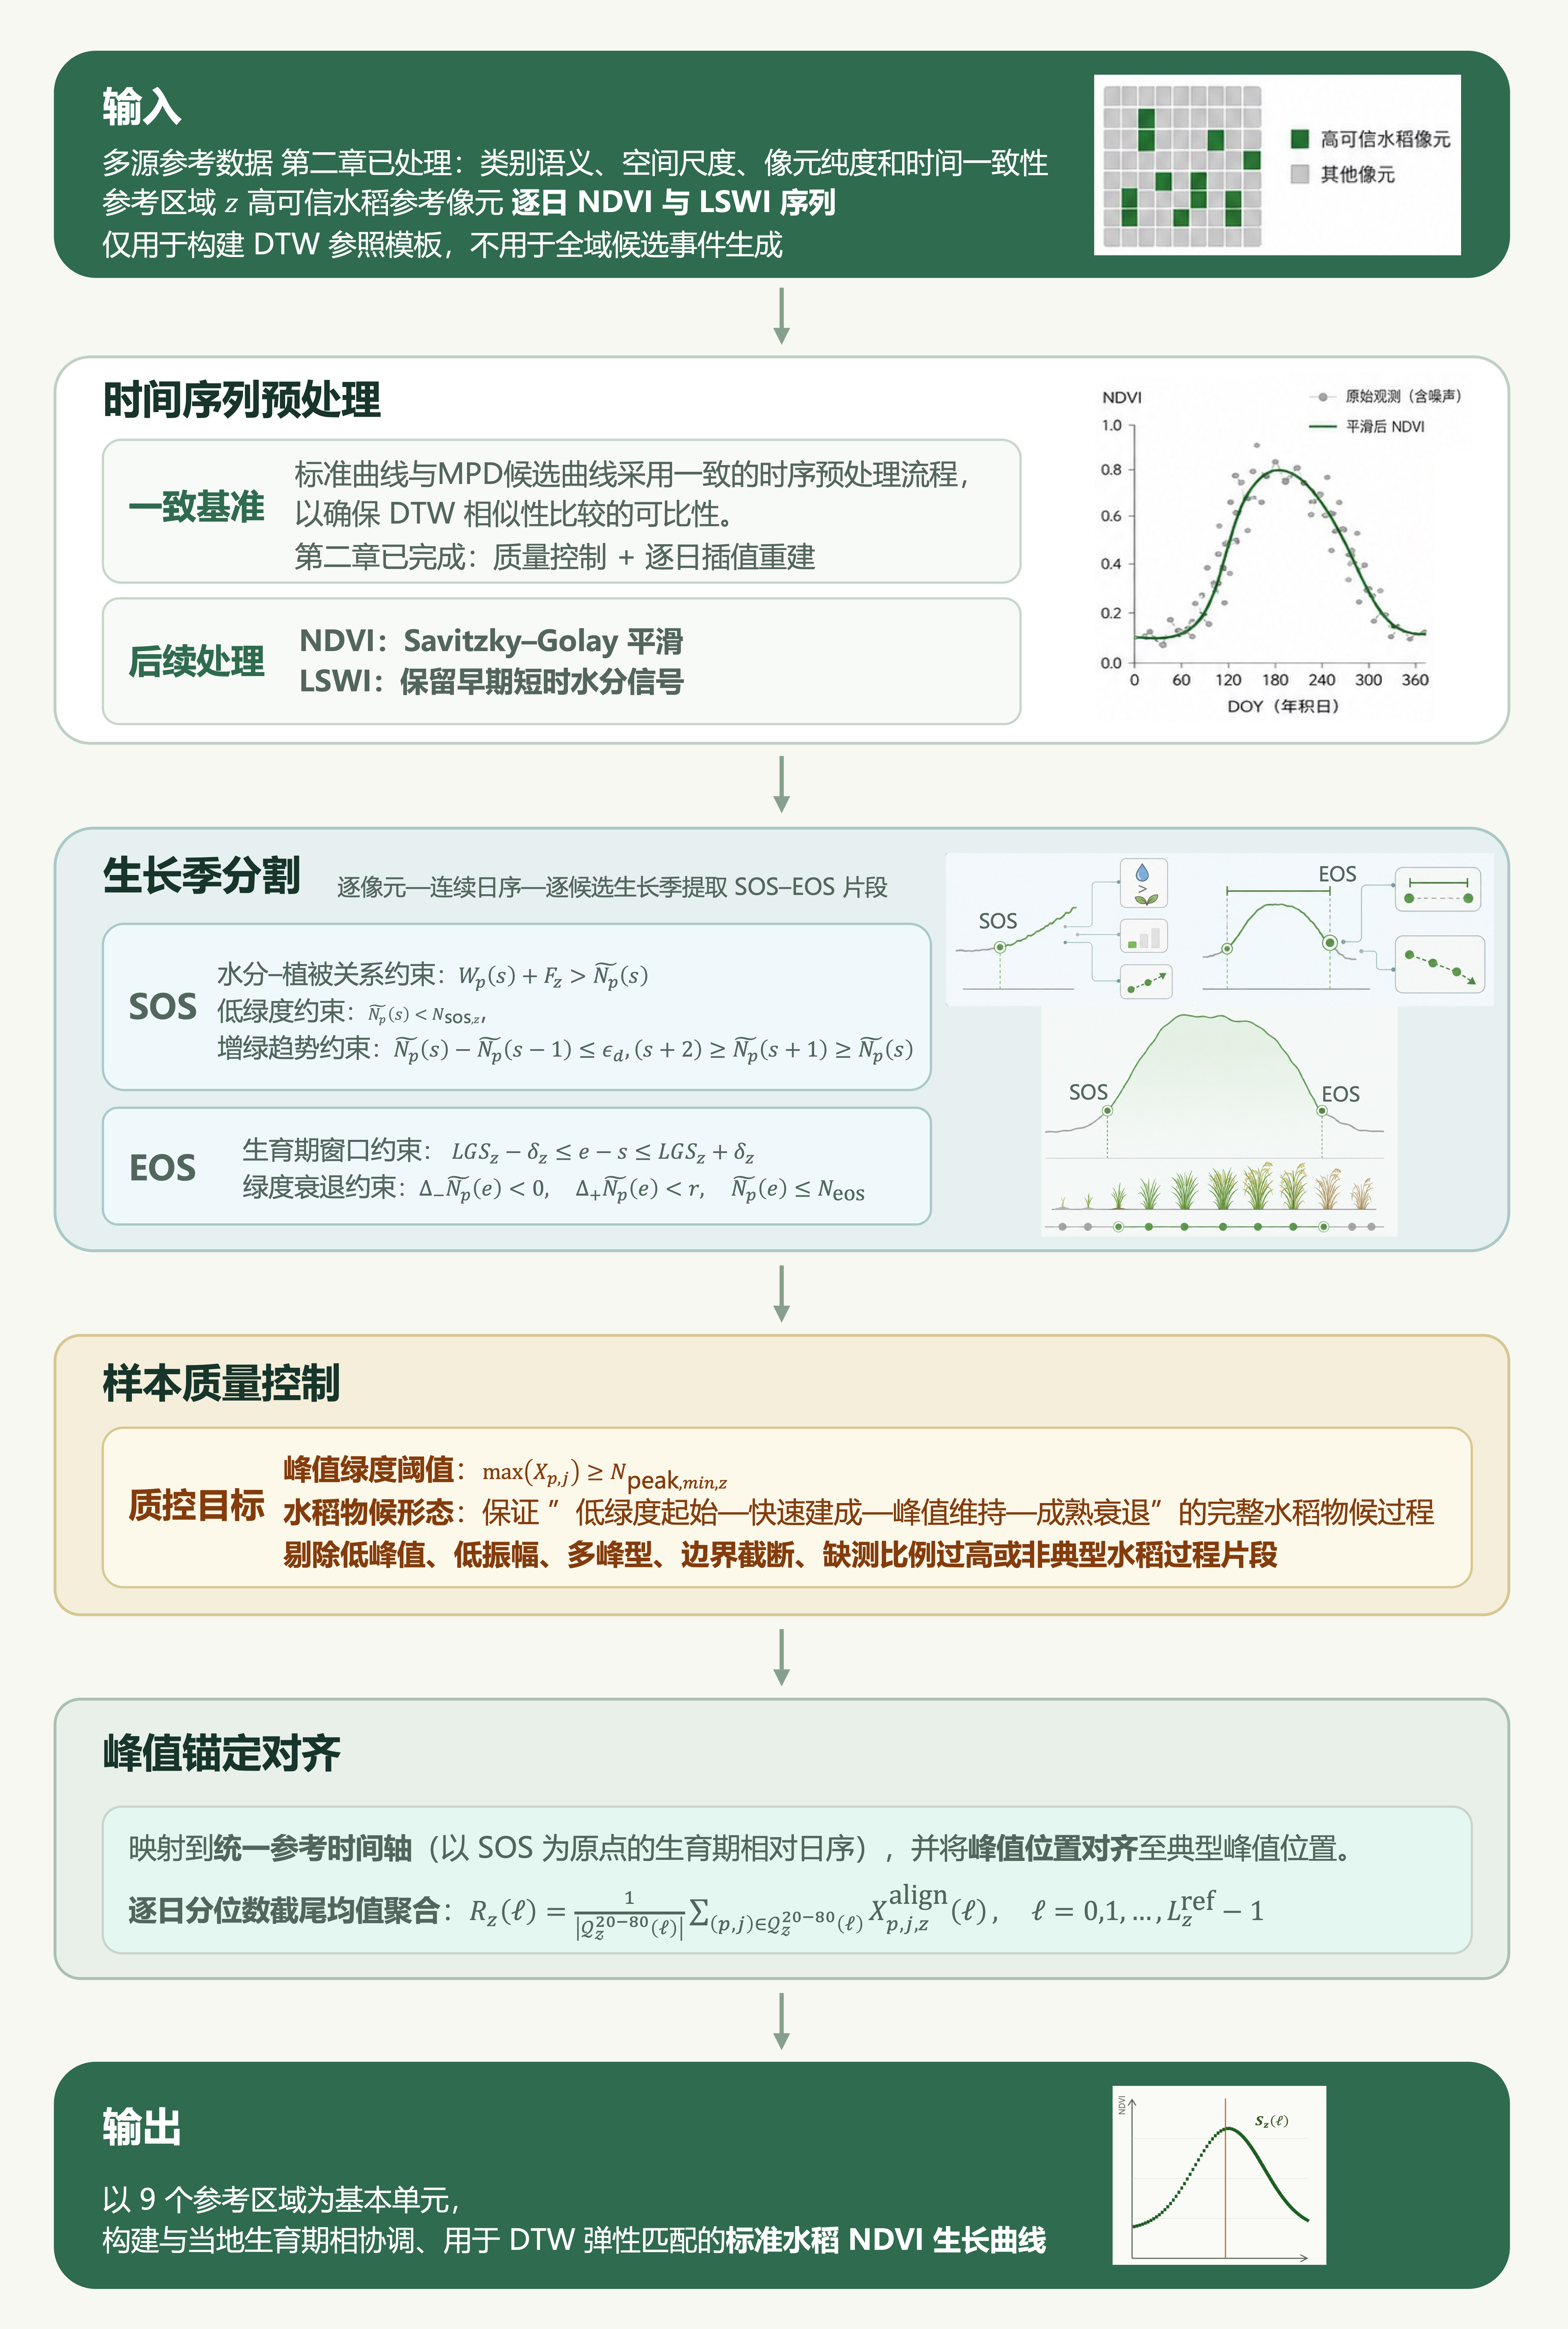
\includegraphics[width=0.99\textwidth]{figure/chapter3/std_curve_workflow.png}
    \bicaption{标准曲线构建流程图}{Workflow of standard curve construction}
    \label{fig:ref_series}
\end{figure}

% 时间序列预处理
在时间序列预处理方面，标准曲线构建与 MPD 候选生长季识别采用一致的日尺度 NDVI 和 LSWI 处理流程，以保证标准曲线和候选曲线在相同数据基准下进行相似性比较。具体而言，日尺度 NDVI 序列采用 Savitzky--Golay 滤波进行平滑，以削弱残余云污染、气溶胶噪声和观测几何差异造成的高频波动，同时尽量保留水稻冠层生长曲线的峰值宽度和总体线型特征\cite{Chen2004RSE}。LSWI 序列主要用于表征水稻移栽或返青初期浅水层、湿润土壤背景和稀疏植被共同作用形成的短时水分信号。为避免平滑处理削弱该水分信号的相对幅度和发生时相，本文使用质量控制和插值重建后的日尺度 LSWI 序列参与水分--植被关系判定，而不再进行额外滤波。

% 生长季分割
在生长季分割方面，标准曲线构建沿用 MPD 模块的基本物候逻辑，即首先依据早期水分--植被组合信号确定候选 SOS，随后基于水稻生长季持续时间的先验范围确定候选 EOS 搜索窗口，并依据成熟期 NDVI 衰退特征搜索候选 EOS。由于这些判据的生物物理基础已在第~\ref{sec:mpd}~节中阐述，本文不再重复完整推导，而重点说明标准曲线样本提取中与样本可靠性相关的保守约束。

候选 SOS 需同时满足三类条件。第一，水分--植被关系约束，用于捕捉水稻移栽或返青初期浅水层、湿润土壤背景与低植被覆盖共同形成的 LSWI 相对增强信号。第二，低绿度约束，用于保证候选起点仍处于低冠层覆盖和低绿色生物量阶段，避免将快速生长期或旺盛生长期误判为生长季起点。第三，增绿趋势约束，用于确认该水分--低绿度信号之后伴随水稻返青、分蘖和冠层快速建成过程，而非短期积水、湿润背景或噪声扰动。

设参数区 \(z\) 内参考像元 \(p\) 在日期 \(t\) 的 LSWI 为 \(W_p(t)\)，平滑 NDVI 为 \(\widetilde{N}_p(t)\)。候选 SOS \(s\) 需满足式 \ref{eq:sos_condition} 中的水分--植被关系约束和低绿度约束，即：
\begin{equation}
    W_p(s)+F_z>\widetilde{N}_p(s), \quad
    \widetilde{N}_p(s)<N_{\mathrm{sos},z},
    \label{eq:std_sos_water_lowgreen}
\end{equation}
其中，\(F_z\) 为参数区 \(z\) 的洪水因子，用于补偿混合像元、弱淹水条件或不同水分管理方式下 LSWI 信号被削弱的问题；\(N_{\mathrm{sos},z}\) 为参数区 \(z\) 的 SOS 阶段 NDVI 上限，用于限定候选起点处于低绿度阶段。此外，候选 SOS 还需满足起点前后的局部趋势约束：
\begin{equation}
    \widetilde{N}_p(s)-\widetilde{N}_p(s-1)\leq \epsilon_d,
    \quad
    \widetilde{N}_p(s+1)\geq \widetilde{N}_p(s),
    \quad
    \widetilde{N}_p(s+2)\geq \widetilde{N}_p(s+1),
    \label{eq:std_sos_trend}
\end{equation}
其中，\(\epsilon_d\) 为起点前局部变化的容差阈值。该约束要求候选 SOS 不位于已经持续增绿的冠层发育阶段，同时要求起点之后 NDVI 出现连续回升，从而提高标准曲线样本起始边界的可靠性。

候选 SOS 确定后，候选 EOS 的搜索（式 \ref{eq:eos_condition}）限定在参数区 \(z\) 的典型水稻生育期范围内。设参数区 \(z\) 的水稻典型生育期长度为 \(LGS_z\)，允许偏差为 \(\delta_z\)，则对于候选 SOS \(s\)，候选 EOS \(e\) 的搜索集合定义为：
\begin{equation}
    \Omega^{\mathrm{std}}_{\mathrm{EOS}}(s)=
    \left\{
    e \mid LGS_z-\delta_z \leq e-s \leq LGS_z+\delta_z
    \right\}.
    \label{eq:std_eos_window}
\end{equation}
其中，\(e-s+1\) 表示由候选 SOS 到候选 EOS 构成的生育期长度，\(LGS_z\) 表示参数区 \(z\) 内水稻从起始期到成熟收获期的典型持续时间，\(\delta_z\) 为允许的生育期长度偏差。该约束用于排除明显短于完整水稻生育过程的短期水分扰动或噪声片段，同时避免截取过长片段而混入休闲期或下一季作物生长信号。

若同一候选 SOS 后存在多个满足成熟期衰退条件且位于 \(\Omega^{\mathrm{std}}_{\mathrm{EOS}}(s)\) 内的候选 EOS，则选择生长季长度最接近参数区典型生育期长度 \(LGS_z\) 的 EOS 作为该参考样本的终点：
\begin{equation}
    e^{*}=
    \arg\min_{e\in\Omega^{\mathrm{std}}_{\mathrm{EOS}}(s)}
    \left| (e-s)-LGS_z \right|.
    \label{eq:std_eos_selection}
\end{equation}
若某一候选 SOS 后不存在同时满足生育期长度约束和成熟期衰退条件的 EOS，或所得 SOS--EOS 片段缺失快速增绿、峰值维持和成熟衰退等关键阶段，则该片段不进入标准曲线样本集。

% 样本质量控制
完成逐像元生长季分割后，本文进一步对参考生长季样本进行质量控制。对于参数区 \(z\) 中由参考像元 \(p\) 提取的第 \(j\) 个生长季片段，记其平滑 NDVI 序列为
\[
    X_{p,j}=\left\{\widetilde{N}_p(t)\mid s_{p,j}\leq t\leq e_{p,j}\right\}.
\]
由于生育期长度约束已在候选 EOS 搜索阶段通过式~\ref{eq:std_eos_window} 实现，质量控制主要从峰值绿度和曲线形态两个方面剔除异常片段。

为保证参考样本具有清晰的水稻冠层发育信号，生长季片段的峰值 NDVI 需达到参数区设定的最小峰值绿度阈值：
\begin{equation}
    \max\left(X_{p,j}\right)\geq N_{\mathrm{peak},\min,z},
    \label{eq:std_peak_threshold}
\end{equation}
其中，\(\max\left(X_{p,j}\right)\) 表示参考像元 \(p\) 的第 \(j\) 个生长季片段内的峰值 NDVI，\(N_{\mathrm{peak},\min,z}\) 为参数区 \(z\) 的最小峰值 NDVI 阈值。该约束用于剔除冠层发育不足、季节性绿度变化不明显或受混合像元影响较强的参考片段。

同时，为保证标准曲线样本能够表征完整且连续的水稻物候过程，本文进一步约束 NDVI 曲线在峰值前后的局部变化方向。设样本片段的峰值日期为
\begin{equation}
    t^{\max}_{p,j}
    =
    \arg\max_{s_{p,j}\leq t\leq e_{p,j}}
    \widetilde{N}_p(t),
    \label{eq:std_peak_date}
\end{equation}
并定义相邻日期的 NDVI 差分为
\begin{equation}
    \Delta\widetilde{N}_p(t)
    =
    \widetilde{N}_p(t+1)-\widetilde{N}_p(t).
    \label{eq:std_ref_derivative}
\end{equation}
质量控制阶段仅保留满足：
\begin{equation}
    \Delta\widetilde{N}_p(t)\geq -\epsilon_w,
    \quad s_{p,j}+5\leq t<t^{\max}_{p,j},
    \label{eq:std_prepeak_smoothness}
\end{equation}
\begin{equation}
    \Delta\widetilde{N}_p(t)\leq \epsilon_w,
    \quad t^{\max}_{p,j}\leq t<e_{p,j},
    \label{eq:std_postpeak_smoothness}
\end{equation}
的生长季片段。其中，\(\epsilon_w\) 为允许的局部波动阈值。式~\ref{eq:std_prepeak_smoothness} 用于保证峰值之前 NDVI 总体呈增绿趋势，并允许移栽或返青初期存在短暂低值波动；式~\ref{eq:std_postpeak_smoothness} 用于保证峰值之后 NDVI 总体呈成熟衰退趋势。由此可剔除受残余噪声、相邻作物季信号或非典型作物过程影响的多峰型片段，使进入标准曲线集合的样本表现为从低绿度起始、冠层快速建成、峰值或高值维持到成熟衰退的典型水稻 NDVI 生长曲线。

% 时间对齐
由于不同参考像元和不同年份的水稻生长季在日历时间上存在物候相位差异，且不同样本的实际生育期长度并不完全一致，若直接按照原始日期对 NDVI 片段进行聚合，容易造成增绿期、峰值期和成熟衰退期的错位叠加，从而削弱标准曲线的阶段边界和典型形态。为降低日历时相差异对模板构建的影响，本研究首先将通过质量控制的 SOS--EOS 参考生长季片段转换为以 SOS 为时间原点的生育期相对日序，随后根据参数区内的典型峰值位置对参考曲线进行整体平移，使不同样本的峰值或高绿度阶段在聚合前具有一致的相对位置（图 \ref{fig:peak_align}）。

\begin{figure}[htbp]
    \centering
    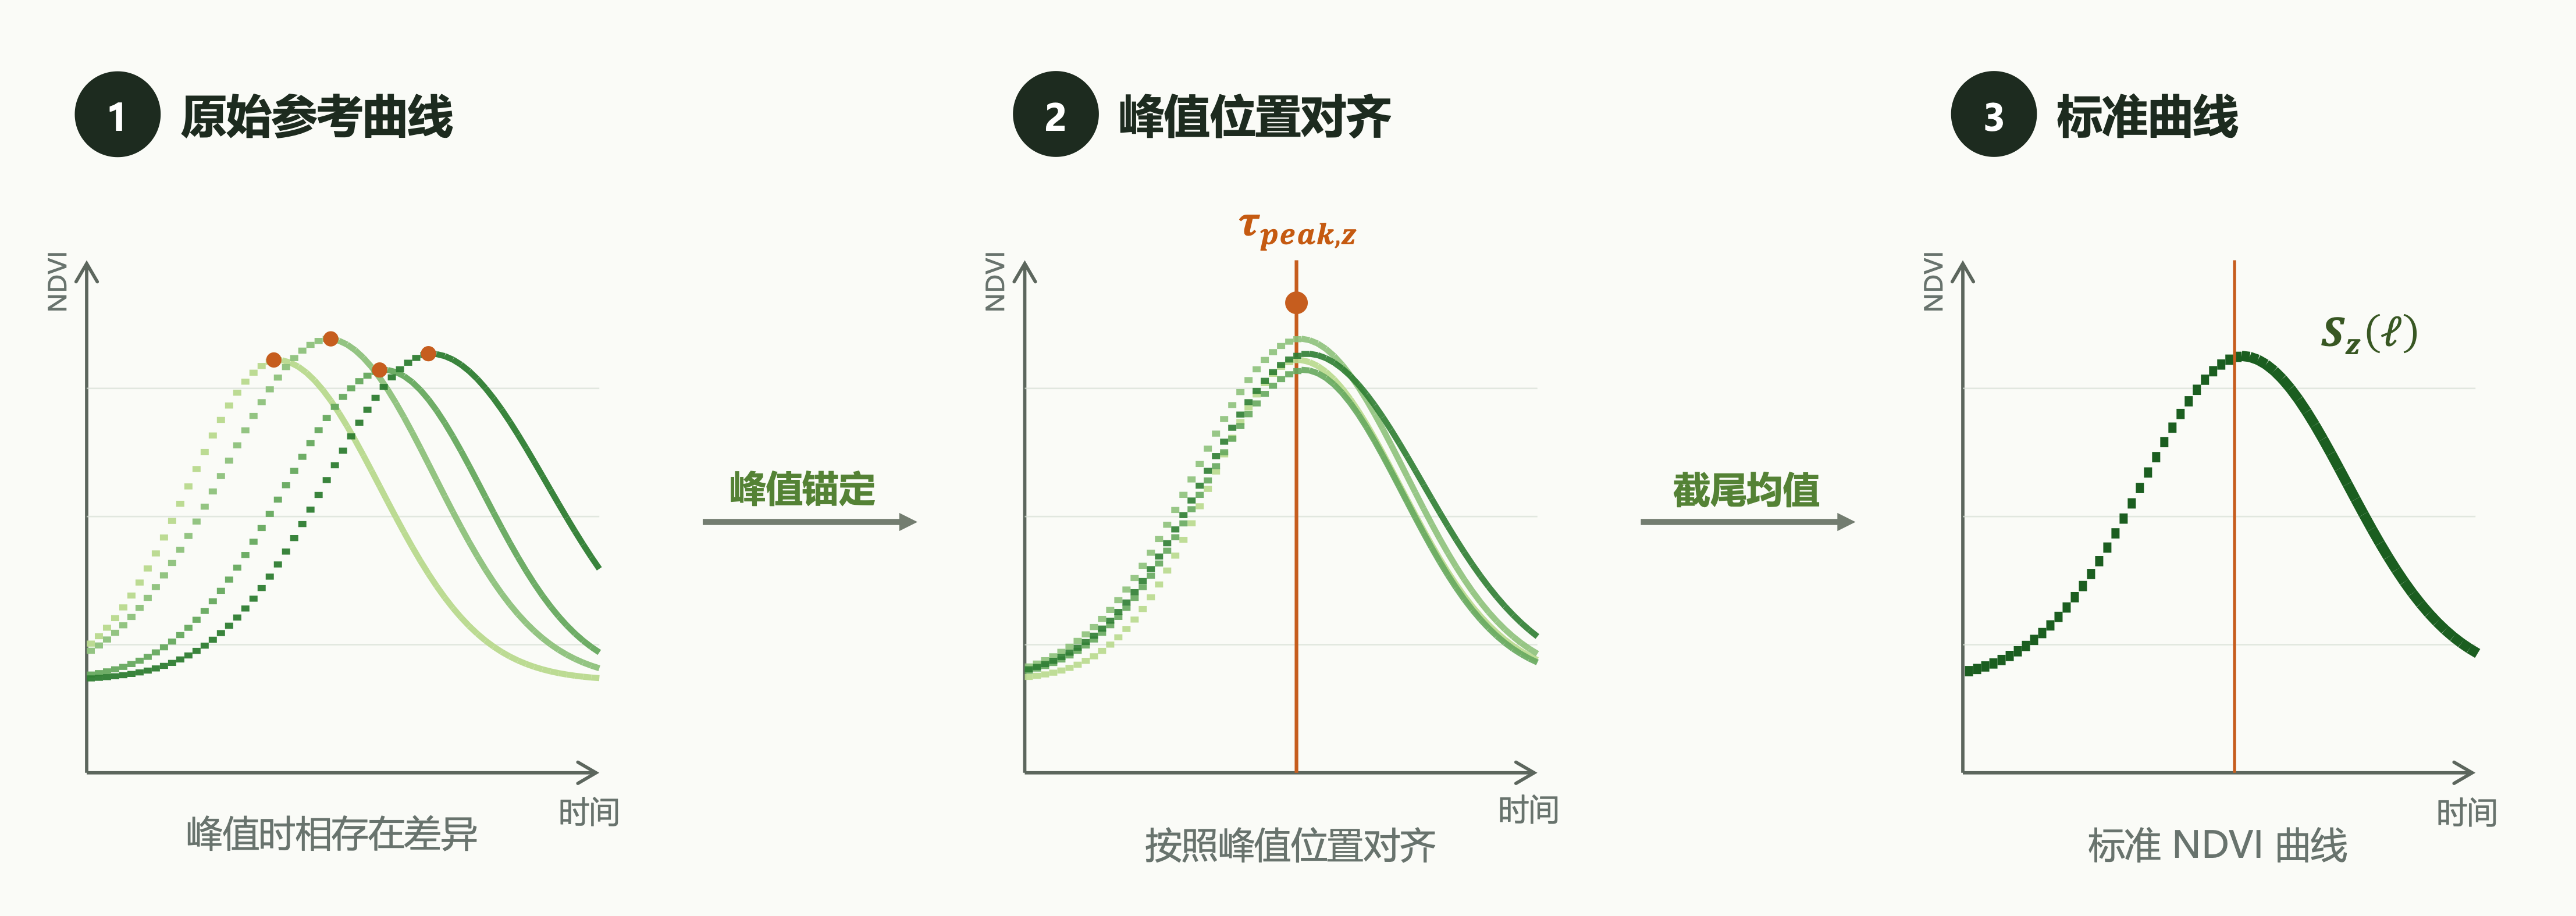
\includegraphics[width=0.99\textwidth]{figure/chapter3/peak_align.png}
    \bicaption{标准水稻生长曲线的峰值锚定对齐与聚合示意图}{Peak-anchored alignment and aggregation of standard rice growth curves}
    \label{fig:peak_align}
\end{figure}

% 统一时间轴：days after SOS
具体而言，对于参数区 \(z\) 中由参考像元 \(p\) 提取的第 \(j\) 个合格生长季片段，记其 SOS 和 EOS 分别为 \(s_{p,j}\) 和 \(e_{p,j}\)。首先以 SOS 为时间原点，将该片段从原始日历时间 \(t\) 转换为生育期相对日序 \(d\)，即
\[
    d=t-s_{p,j}, \quad d=0,1,\ldots,L_{p,j}-1,
\]
其中 \(L_{p,j}=e_{p,j}-s_{p,j}+1\) 为该参考片段的实际长度。转换后的 NDVI 曲线记为
\[
    X^{\mathrm{SOS}}_{p,j,z}(d)
    =
    \widetilde{N}_p(s_{p,j}+d),
    \quad d=0,1,\ldots,L_{p,j}-1 .
\]
该处理使所有参考样本首先被表达在同一类相对时间基准上，即 SOS 后天数（days after SOS），从而消除不同年份和不同像元之间因播栽日期差异造成的日历时相偏移。

% 按照峰值对齐
随后提取每条参考曲线在生育期相对日序上的峰值位置：
\[
    d^{\max}_{p,j}
    =
    \arg\max_{0\leq d<L_{p,j}}
    X^{\mathrm{SOS}}_{p,j,z}(d).
\]
参数区 \(z\) 的典型峰值位置记为 \(d^{\mathrm{ref}}_z\)，可由先验物候参数指定，或由该区合格参考样本峰值位置的统计结果确定。以 \(d^{\mathrm{ref}}_z\) 作为峰值锚点，对每条参考曲线进行整体平移。对于样本 \((p,j)\)，其平移量定义为
\[
    \Delta_{p,j,z}
    =
    d^{\mathrm{ref}}_z-d^{\max}_{p,j}.
\]
完成峰值锚定后的参考曲线可表示为
\[
    X^{\mathrm{align}}_{p,j,z}(\ell)
    =
    X^{\mathrm{SOS}}_{p,j,z}(\ell-\Delta_{p,j,z}),
\]
其中 \(\ell=0,1,\ldots,L^{\mathrm{ref}}_z-1\) 表示峰值锚定后的统一参考时间轴位置，\(L^{\mathrm{ref}}_z\) 为参数区 \(z\) 内用于标准曲线聚合的参考序列长度。只有当
\[
    0\leq \ell-\Delta_{p,j,z} \leq L_{p,j}-1
\]
时，\(X^{\mathrm{align}}_{p,j,z}(\ell)\) 才对应于该样本实际 SOS--EOS 片段内的有效 NDVI 值；对于平移后超出样本实际长度或统一参考时间轴范围的位置，不进行外推补值，而是在后续逐位置聚合时作为无效值处理。

峰值锚定对齐在每条参考曲线已经转换为生育期相对日序后进行。该处理一方面保留了每个水稻生长季片段从低绿度起始、冠层快速建成、峰值或高值维持到成熟衰退的相对物候结构，另一方面减少了不同播栽日期、不同年份和不同区域管理差异对标准曲线聚合的影响。

% 均值聚合：20-80% 分位数截尾均值
为进行稳健聚合，记参数区 \(z\) 内通过质量控制并完成峰值锚定对齐的参考生长季样本集合为 \(\mathcal{Q}_z\)。对于统一参考时间轴上的任一位置 \(\ell\)，仅保留在该位置具有有效 NDVI 值的参考样本，构成有效样本集合：
\[
    \mathcal{V}_{z}(\ell)
    =
    \left\{
    (p,j)\in\mathcal{Q}_z
    \mid
    0\leq \ell-\Delta_{p,j,z} \leq L_{p,j}-1
    \right\}.
\]
随后基于 \(\mathcal{V}_{z}(\ell)\) 中的有效样本值计算第 20 百分位数和第 80 百分位数：
\[
    P_{20,z}(\ell)
    =
    \mathrm{percentile}_{20}
    \left\{
    X^{\mathrm{align}}_{p,j,z}(\ell)
    \mid
    (p,j)\in\mathcal{V}_{z}(\ell)
    \right\},
\]
\[
    P_{80,z}(\ell)
    =
    \mathrm{percentile}_{80}
    \left\{
    X^{\mathrm{align}}_{p,j,z}(\ell)
    \mid
    (p,j)\in\mathcal{V}_{z}(\ell)
    \right\}.
\]
在每一个对齐时间位置 \(\ell\)，剔除低于第 20 百分位数和高于第 80 百分位数的样本值，仅保留位于该分位数范围内的参考样本：
\[
    \mathcal{Q}^{20-80}_{z}(\ell)
    =
    \left\{
    (p,j)\in\mathcal{V}_{z}(\ell)
    \mid
    P_{20,z}(\ell)
    \leq
    X^{\mathrm{align}}_{p,j,z}(\ell)
    \leq
    P_{80,z}(\ell)
    \right\}.
\]
参数区 \(z\) 的标准 NDVI 生长曲线定义为逐位置的 20--80\% 分位数截尾均值：
\begin{equation}
    R_z(\ell)
    =
    \frac{1}{|\mathcal{Q}^{20-80}_{z}(\ell)|}
    \sum_{(p,j)\in\mathcal{Q}^{20-80}_{z}(\ell)}
    X^{\mathrm{align}}_{p,j,z}(\ell),
    \quad
    \ell=0,1,\ldots,L^{\mathrm{ref}}_z-1 .
    \label{eq:std_curve}
\end{equation}
其中，\(\mathcal{V}_{z}(\ell)\) 表示在对齐时间位置 \(\ell\) 上具有有效 NDVI 值的参考样本集合，\(\mathcal{Q}^{20-80}_{z}(\ell)\) 表示在该位置剔除低于第 20 百分位数和高于第 80 百分位数样本值后保留的参考样本集合，\(|\mathcal{Q}^{20-80}_{z}(\ell)|\) 为该位置参与均值计算的样本数量。分位数截尾均值聚合方法能够在保留区域内多数合格参考样本平均物候特征的同时，降低残余异常值、局部管理差异、混合像元影响或少量非典型曲线对标准模板形态的干扰。最终得到的 \(R_z\) 即为参数区 \(z\) 的标准水稻 NDVI 生长曲线，并作为后续 DTW 模块判别候选 SOS--EOS 片段是否符合区域典型水稻生育过程的参照模板。

% 各参考区域的标准曲线
\begin{figure}[htbp]
    \centering
    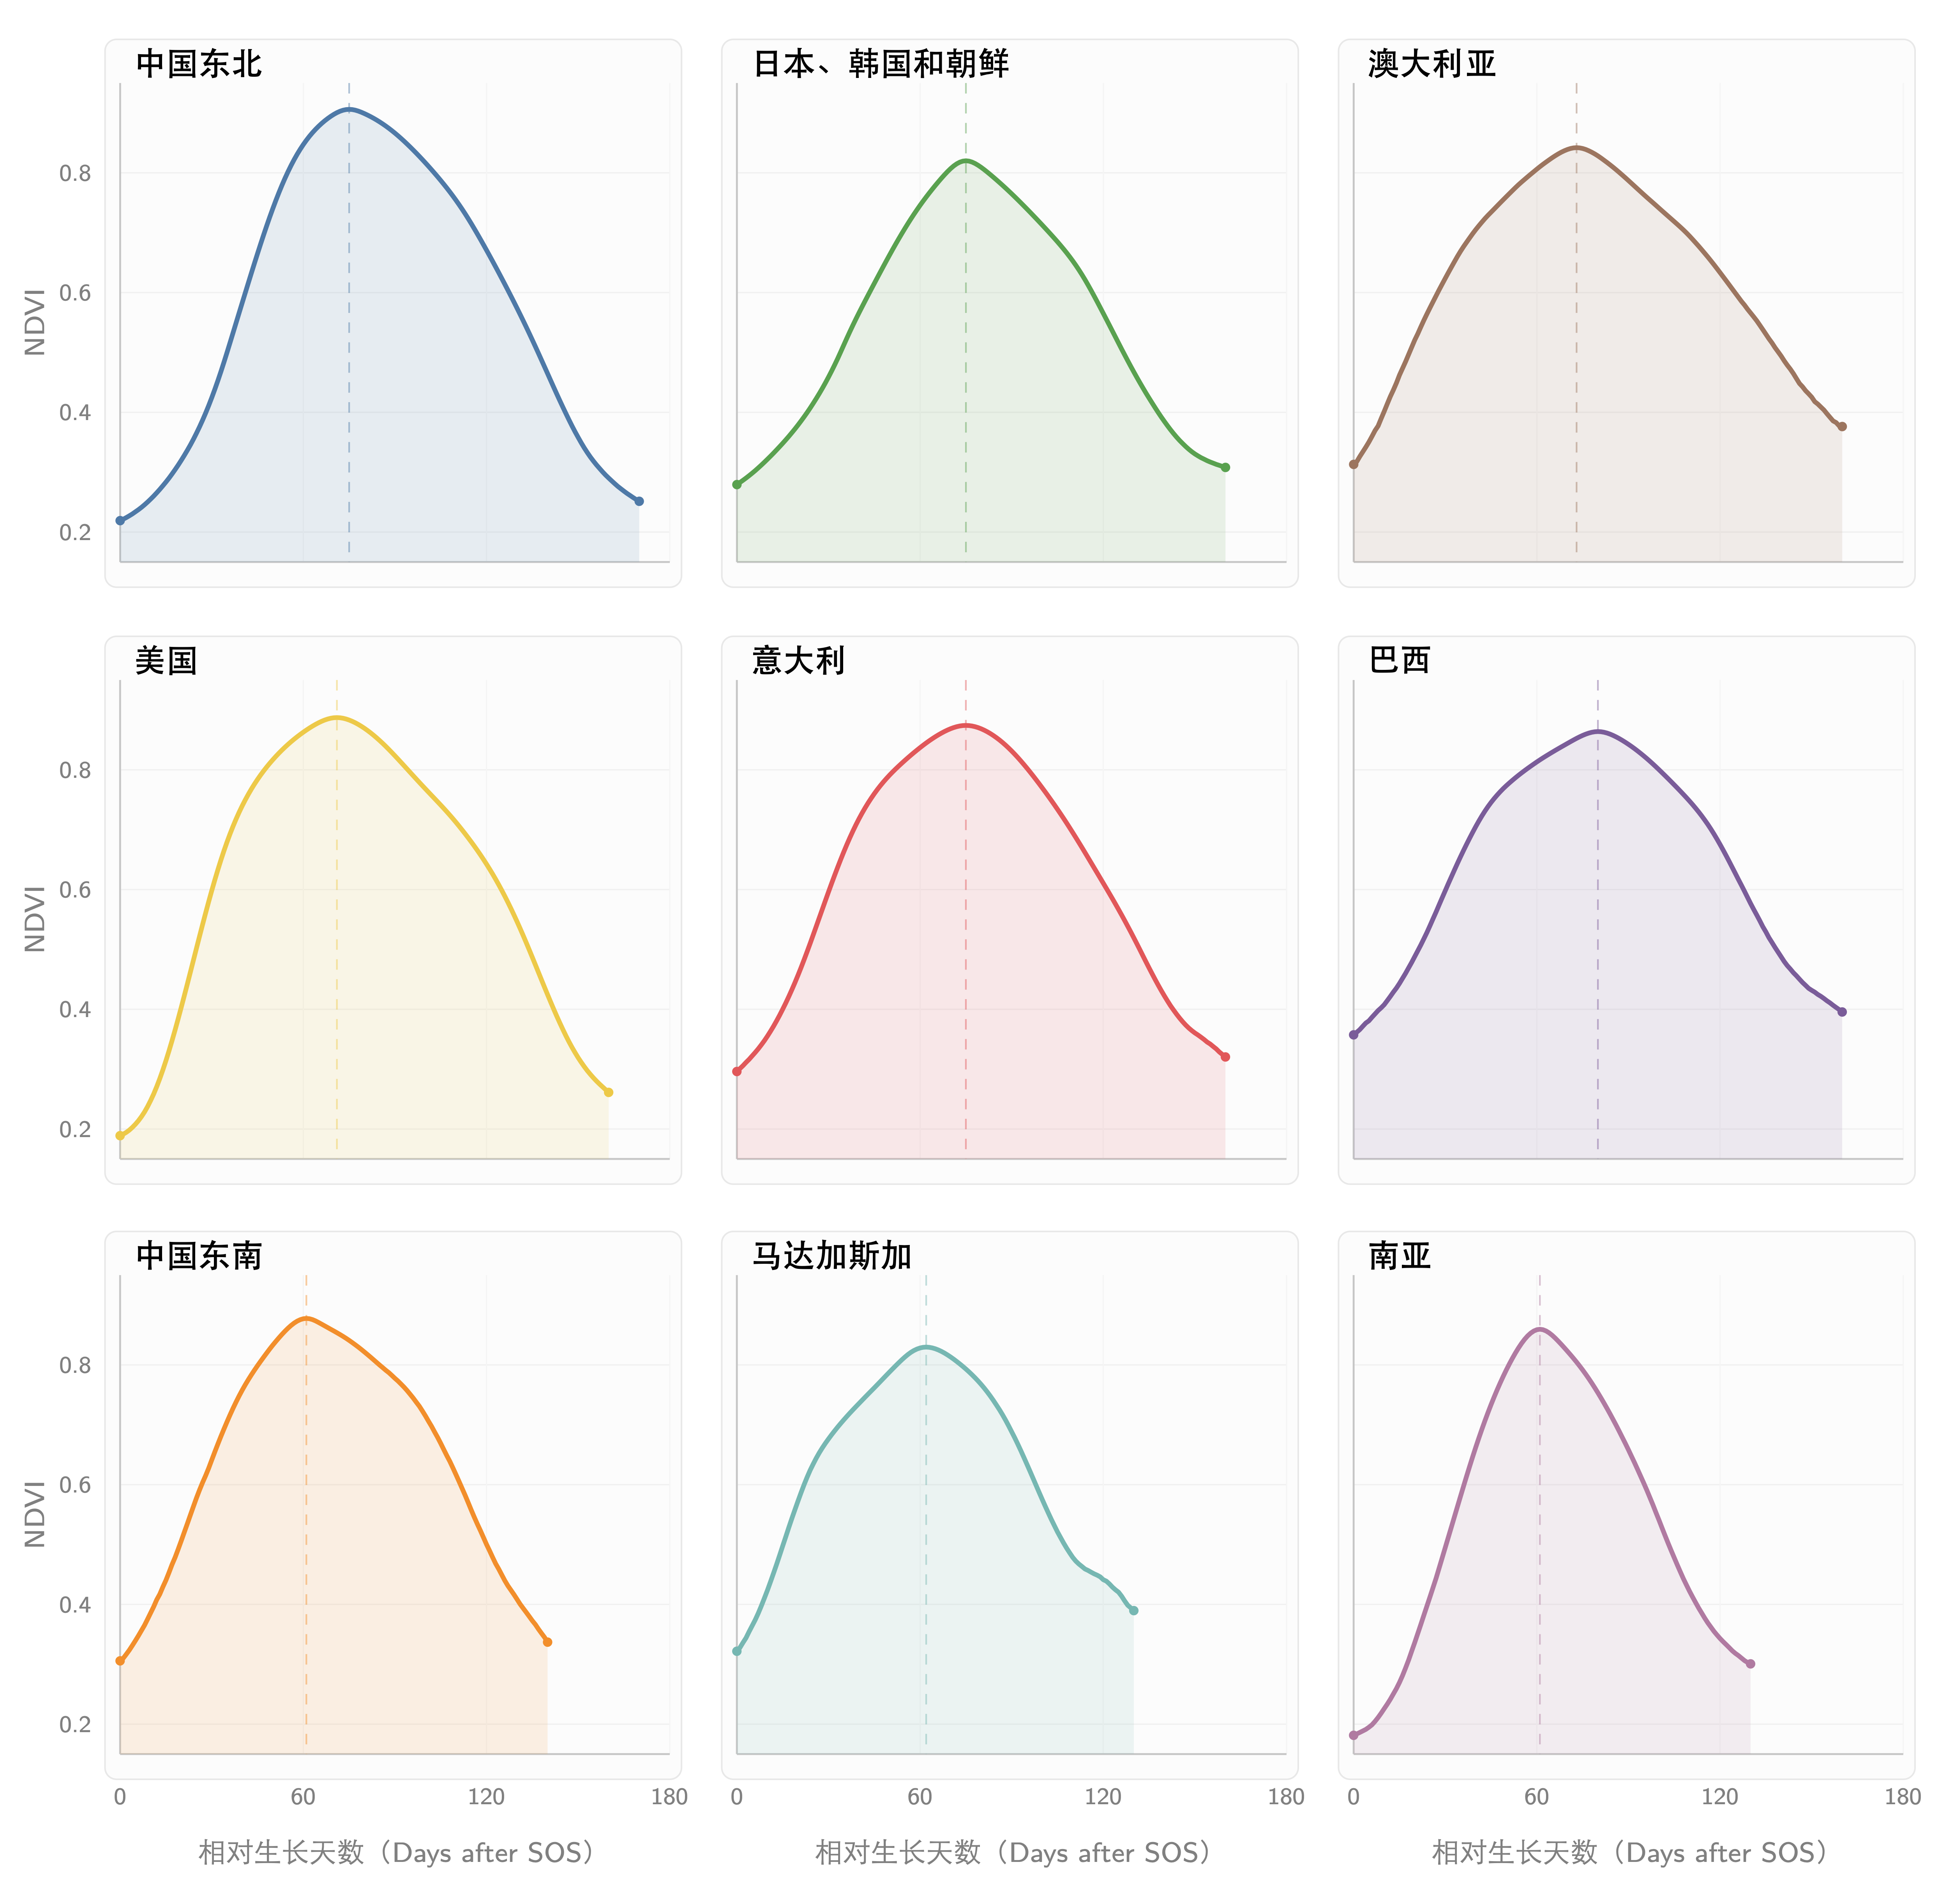
\includegraphics[width=0.99\textwidth]{figure/chapter3/standard_curves.png}
    \bicaption{参考区域标准水稻曲线}{Standard rice curves for each reference region}
    \label{fig:standard_curves}
\end{figure}

全球水稻种植制度在气候背景、品种类型、播栽制度和生育期长度上具有显著区域差异 \cite{Laborte2017SciData}。若采用单一全球标准曲线，不同稻区的真实物候节律将被压缩到同一时间尺度内，容易使 DTW 规整路径产生缺乏农学含义的时间拉伸或压缩，进而削弱曲线匹配结果的物候解释性 \cite{Guan2016RemoteSensing}。
基于此考虑，本研究构建区域化日尺度 NDVI 标准曲线集合，使候选水稻曲线能够在与当地生育期相协调的时间尺度内进行弹性匹配，从而提高 MPD\_DTW 判别过程对不同稻作制度的适应能力。

标准水稻曲线以第二章所述 9 个参考区域为基本单元分别构建。在每个参考区域内，本研究基于高可信水稻参考像元提取日尺度 NDVI 生长季片段，按照前述样本筛选、峰值锚定对齐和分位数截尾均值聚合流程生成对应的区域标准曲线，如图 \ref{fig:standard_curves} 所示。
由此形成的区域化标准曲线集合能够表征各参考区域内典型水稻 NDVI 生长过程，并保留不同稻区在生长季长度、峰值出现时间、增绿速率和成熟期衰退过程等方面的关键物候差异。在后续候选生长季判别中，候选 SOS--EOS 片段将与对应区域的标准曲线进行相似性匹配，以判断其是否符合当地水稻从建植、生长到成熟收获的典型物候轨迹。

\subsection{基于 MPD\_DTW 的水稻生长季事件连续识别}

\label{sec:feedback}

% MPD_DTW连续识别的设计背景
全球水稻种植制度具有显著的时空异质性，同一像元在一年内可能仅经历一次水稻生长季，也可能连续经历双季或多季水稻；在部分热带和南半球地区，水稻生长过程可能跨越自然年边界。
因此，全球水稻遥感制图的关键并不仅在于判断某一像元是否种植水稻，还在于沿连续时间轴识别每一次完整的水稻生长季事件。
MPD\_DTW 框架正是围绕这一目标构建，其核心思想是先基于水稻物候特征确定候选生长季边界，再利用完整绿度演化过程确认该候选片段是否对应真实水稻生长季，并通过反馈机制连续推进后续事件识别。

前述 MPD 模块（第 \ref{sec:mpd} 节）和 DTW 模块（第 \ref{sec:dtw} 节）分别解决了候选季节边界生成和水稻生长过程判别两个问题。
MPD 模块根据水稻关键物候阶段的遥感光谱响应特征，在逐日 NDVI--LSWI 时间序列中动态识别候选 SOS--EOS 边界，为后续判别提供具有物候意义的时间片段。
DTW 模块则在候选 SOS--EOS 区间内比较 NDVI 曲线与标准水稻曲线之间的形态相似性，重点检验候选生长季是否呈现水稻生长过程中绿度上升、峰值维持以及成熟收获后衰减的连续演化特征。
通过边界定位与过程匹配的耦合，MPD\_DTW 将局部物候信号组织为完整生长季事件的识别依据，使水稻季节判别同时受到物候边界和生长曲线形态的约束。

MPD\_DTW 的连续识别能力来自 MPD 与 DTW 之间的反馈推进机制。
在每一次候选生长季判别后，DTW 结果不仅决定当前候选片段是否被记录为水稻生长季，也决定下一轮候选 SOS 搜索在时间轴上的起点。
这种反馈机制使算法能够在同一像元内依次识别多个水稻生长季事件，并避免将单个候选片段的判别结果孤立处理。

\begin{figure}[htbp]
    \centering
    
\includegraphics[width=0.99\textwidth]{figure/chapter3/mpd_dtw_feedback.png}
    \bicaption{MPD\_DTW 反馈机制流程图}{Feedback mechanism of MPD\_DTW}
    \label{fig:mpd_dtw_feedback}
\end{figure}

设当前候选 SOS 为 \(s\)。在满足区域生长期长度约束的候选 EOS 集合中，DTW 模块计算所有候选生长季 \((s,e)\) 与标准水稻曲线之间的 DTW 距离。距离最小的候选生长季为最优候选生长季 \((s,e^{*})\)，其对应距离记为 \(d_z(s,e^{*})\)，其中 \(z\) 表示区域化标准曲线或参数分区，\(\theta_z\) 为该分区对应的 DTW 判别阈值。
当 \(d_z(s,e^{*})<\theta_z\) 时，候选片段被确认为一次水稻生长季事件，并记入当前像元的水稻事件序列。
此时，下一轮 SOS 搜索从该季 EOS 之后开始：
\begin{equation}
    t_{\mathrm{next}}=e^{*}+1,\quad \mathrm{if}\ d_z(s,e^{*})<\theta_z.
    \label{eq:positive_feedback}
\end{equation}
该正向反馈使得已经确认的水稻生长季在时间轴上形成完整事件单元。后续搜索从该季 EOS 之后继续，可以避免同一生长过程被重复识别，并保证相邻水稻季之间具有明确的时间顺序。
对于双季稻和多季稻像元，前一季水稻收获后，算法继续在后续时间序列中搜索新的候选 SOS；若新的候选片段再次满足 MPD 边界条件和 DTW 曲线形态条件，则被记录为同一像元内的下一次水稻生长季事件。
由此，MPD\_DTW 能够将像元级水稻种植过程表达为按时间顺序排列的事件序列，而非单一的年度水稻标记。

该负向反馈策略在剔除当前非水稻候选片段的同时，保留了对邻近时间段真实水稻季的搜索能力，可降低短期积水、湿地植被变化、噪声波动或非水稻作物局部相似曲线造成的漏检风险。

当 \(d_z(s,e^{*})\geq\theta_z\) 时，当前候选片段未通过水稻生长过程判别。
该片段可能包含局部水分增强、短期绿度波动或类似成熟收获的下降信号，但其完整 NDVI 曲线形态与标准水稻生长过程不一致。
若此时直接跳过整个候选片段，真实水稻季可能因邻近的非水稻候选事件而被遗漏。
因此，MPD\_DTW 采用负向反馈，将下一轮搜索位置推进至当前 SOS 之后：
\begin{equation}
    t_{\mathrm{next}}=s+1,\quad \mathrm{if}\ d_z(s,e^{*})\geq\theta_z.
    \label{eq:negative_feedback}
\end{equation}
该负向反馈保留了对邻近时间段真实水稻季的搜索能力。
在连续时间序列中，短期积水、湿地植被变化、遥感噪声或非水稻作物的局部相似变化均可能触发候选 SOS。
MPD\_DTW 在否定当前候选片段后继续向后搜索，使这些局部扰动不会阻断后续真实水稻生长季的识别。
因此，正向反馈和负向反馈共同构成了 MPD\_DTW 连续识别的核心：前者保证已确认水稻季不被重复计数，后者保证未确认候选片段不会过度占用时间轴。

在这一框架下，单季稻、多季稻和跨年稻均可统一理解为连续时间轴上的水稻生长季事件。
单季稻像元通常只记录一次满足 MPD\_DTW 条件的 SOS--EOS 事件；多季稻像元则可能记录多个按时间顺序排列的 SOS--EOS 事件。
对于跨越自然年边界的水稻生长过程，MPD\_DTW 的判别对象仍然是完整的生长季事件，而非被自然年截断的年度片段。
因此，自然年仅作为数据组织和年度产品表达的时间单位，水稻生长季识别则以连续物候过程为基本单位。
这一处理使不同半球、不同种植制度和不同复种强度下的水稻生长过程能够在统一的事件识别框架中表达。

综上，MPD\_DTW 通过 MPD 的物候边界定位、DTW 的完整曲线过程确认和基于判别结果的反馈推进，将逐日遥感时间序列中的局部水分--绿度变化组织为连续水稻生长季事件序列。
该机制使得 MPD\_DTW 生产的水稻数据不仅能够提供年度水稻空间分布，还能够记录逐像元水稻生长季事件及其 SOS--EOS 边界，为全球水稻收获面积统计、复种强度估算和生长季尺度的稻田地表温度效应分析提供统一的时序基础。

\subsection{MPD\_DTW 参数优选策略}
\label{sec:param_selection}

% 总述校准目标
前述章节已分别介绍 MPD\_DTW 的候选生长季事件检测、DTW 曲线匹配判别和反馈式连续识别机制。本节在此基础上建立区域化参数优选策略，旨在统一识别框架下确定适用于不同参数区的参数组合，使 MPD\_DTW 能够适应全球不同稻作制度、农业气候背景和遥感观测条件下的水稻动态识别任务，并在全球尺度制图中兼顾候选水稻生长季的物候合理性、跨区域可迁移性和长期面积稳定性。由于全球水稻种植区在气候背景、播栽方式、生长季长度和复种制度等方面存在显著差异，单一固定参数难以支撑从温带单季稻区到热带多熟稻区的连续识别。因此，本研究结合第~\ref{sec:ref_regions}~节所述九个全球典型参考区域，综合考虑水稻生长季事件识别的完整性、非水稻耕地误识别的控制效果以及候选曲线与标准水稻曲线的匹配程度，分别为各参数区确定最优参数组合。

% 辅助稳定参数
根据参数确定方式和敏感性，可将其划分为辅助稳定参数和核心校准参数两类。
辅助稳定参数主要用于约束候选生长季的时间结构和物候合理性，其取值可依据区域农业气候背景、水稻生育周期和时间序列特征进行先验设定，在不同区域间具有相对稳定的物候含义。该类参数包括 SOS 搜索窗口 $\Omega_{SOS,z}$、生长季长度约束 $T_{\min,z}$--$T_{\max,z}$、EOS 阶段 NDVI 上限 $N_{eos}$、EOS 趋稳速率阈值 $r$ 以及最晚 EOS 尾部约束等。以 SOS 搜索窗口 $\Omega_{SOS,z}$ 为例，温带单季稻区受热量季节性限制，水稻播栽期通常集中于春末至初夏，因而可通过区域化时间窗口限定候选 SOS 的搜索范围，减少积雪融化、非生长季湿润背景或其他非水稻物候过程造成的误判，并提高大范围逐日搜索的计算效率。热带和亚热带多熟区全年水热条件较为充足，水稻播栽时间灵活，固定月份窗口容易遗漏错季种植或连续轮作条件下的真实水稻生长季，因此采用全年移动搜索以增强算法对复杂复种制度的适应性。上述参数在前文机制介绍时已结合水稻物候过程和农业气候背景知识给出经验性设定依据，本节不再重复展开。

% 核心校准参数：洪水因子 \(F_z\)、DTW 距离阈值 \(\theta_z\)
核心校准参数主要包括洪水因子 $F_z$ 和 DTW 距离阈值 $\theta_z$。
与辅助稳定参数相比，$F_z$ 和 $\theta_z$ 对区域稻作制度、农业气候背景、田间水分管理、田块破碎程度、混合像元状况和时序噪声更为敏感，是 MPD\_DTW 分区参数优选的重点对象。
洪水因子 $F_z$ 用于调节水稻移栽或返青初期淹水信号的判别敏感性，直接影响真实水稻生长季能否进入候选集合；其适宜范围受灌溉方式、直播或移栽制度、田面水层维持时间、田块破碎程度和 MODIS 500 m 混合像元效应等因素共同影响。
DTW 距离阈值 $\theta_z$ 用于限定候选 SOS--EOS 时段内实际 NDVI 曲线与区域标准水稻曲线之间可接受的形态差异，直接影响候选生长季能否被确认为水稻生长季；其适宜范围与热量条件、品种熟期、生长季长度、复种制度和时间序列质量密切相关。
二者分别影响候选 SOS 的触发和候选生长季的确认，共同决定水稻制图中的漏分与错分平衡，因此需要在不同参数区内结合参考样本进行重点优选。

% 参考样本的来源（第二章已经预处理）
参数优选所使用的参考样本来源于第~\ref{sec:ref_data}~节构建的 500 m 像元级水稻与非水稻样本库。该参考数据体系覆盖中国东北、中国东南、韩国与日本、东南亚、澳大利亚、马达加斯加、意大利伦巴第、美国和巴西南里奥格兰德州等九个典型参考区域，涵盖单季稻、双季稻和多季稻等主要稻作制度，能够表征不同农业气候背景、田块形态和水分管理条件下的水稻空间分布与时序特征。正样本用于表征具有明确水稻主导特征的像元，负样本来自耕地掩膜内明确的非水稻作物、轮作农田或休耕农田等易与水稻发生混淆的耕地背景。

% 正负样本比例
在大范围水稻遥感制图中，非水稻作物像元通常远多于水稻像元，类别比例不均衡是算法实际运行时必须面对的基本情景。若在参数优选阶段人为构建过度均衡的水稻与非水稻样本比例，精度评价将偏离真实耕地背景，并可能导致参数组合对非水稻误识别风险的估计不足。Xiao 等针对遥感制图测试集样本比例的研究表明，当测试集正负样本比例与目标区域实际分布一致时，用户精度（UA）、F1 值和总体精度（OA）更接近真实水平；若正样本比例被人为抬高，UA、F1 和 OA 将出现系统性高估，而生产者精度（PA）受影响相对较小 \cite{Xiao2024JAG}。这一认识同样适用于本文的参数优选过程。MPD\_DTW 在耕地掩膜内运行，参数优选样本的负正比例应尽量反映参考区域内水稻与其他作物的真实面积关系。

基于上述原则，本研究以参考区域为单元，结合区域耕地背景和统计面积信息确定负正样本比例（negative--positive ratio, $\mathrm{np\_ratio}$），并据此从样本库中选取参与参数比较的水稻与非水稻样本。各参考区域的 $\mathrm{np\_ratio}$ 见表~\ref{tab:mpd_dtw_parameters}。不同参考区域之间的 $\mathrm{np\_ratio}$ 差异反映了水稻在区域耕地结构中的相对占比及复种制度差异：水稻集中分布且耕地背景以旱作作物为主的区域通常具有较高的 $\mathrm{np\_ratio}$，水稻占比较高或复种指数较高的区域则表现出较低的 $\mathrm{np\_ratio}$。
基于 $\mathrm{np\_ratio}$ 构建参数优选样本，能够使样本类别构成更接近算法实际运行时面对的耕地背景，从而降低由样本比例失真引起的参数偏差。

% 评价指标
参数评价采用生产者精度（Producer Accuracy, PA）、用户精度（User Accuracy, UA）、总体精度（Overall Accuracy, OA）和 F1 值进行综合表征，计算公式如下：
\begin{equation}
    \mathrm{PA}=\frac{\mathrm{TP}}{\mathrm{TP}+\mathrm{FN}},\label{eq:PA}
\end{equation}
\begin{equation}
    \mathrm{UA}=\frac{\mathrm{TP}}{\mathrm{TP}+\mathrm{FP}},\label{eq:UA}
\end{equation}
\begin{equation}
    \mathrm{OA}=\frac{\mathrm{TP}+\mathrm{TN}}{\mathrm{TP}+\mathrm{FN}+\mathrm{FP}+\mathrm{TN}},
    \label{eq:OA}
\end{equation}
\begin{equation}
    \mathrm{F1}=\frac{2\times\mathrm{UA}\times\mathrm{PA}}{\mathrm{UA}+\mathrm{PA}}.
    \label{eq:F1}
\end{equation}
其中，TP 表示水稻样本被正确识别为水稻，TN 表示非水稻样本被正确识别为非水稻，FP 表示非水稻样本被误识别为水稻，FN 表示水稻样本被遗漏。PA 主要反映真实水稻生长季的检出能力，UA 主要反映水稻识别结果的可靠性，F1 值综合表征水稻类别的识别效果，OA 用于评价参数区内水稻与非水稻耕地的整体分类一致性。考虑到非水稻耕地在多数参数区内占比较高，单独依赖 OA 容易掩盖水稻类别的漏分或错分问题，因此本文将 PA--UA 平衡和 F1 值作为核心判据，并将 OA 作为整体稳定性的辅助指标。

% 迭代式参数优选策略
在每个参考区域内，本研究采用迭代式策略确定洪水因子 $F_z$ 和 DTW 距离阈值 $\theta_z$ 两个核心校准参数。
参数优选的主要目标是在真实水稻检出和非水稻耕地误识别控制之间取得平衡，即在生产者精度（PA）和用户精度（UA）之间形成合理权衡。
PA 偏低通常表明真实水稻生长季存在漏分，UA 偏低则说明非水稻耕地被错分为水稻的比例较高。因此，参数优选不单独追求某一项精度指标的最大值，而是综合比较 PA、UA、F1 和 OA 的变化，选择能够稳定表达区域水稻物候特征并有效控制非水稻混淆的参数组合。

具体而言，本研究在各参考区域内采用逐步迭代的方式确定 $F_z$ 和 $\theta_z$。迭代过程以 $F_z=0$ 作为基准淹水判别条件，并在此基础上逐步增加洪水因子，以考察淹水信号判别条件放宽后候选 SOS 集合及后续水稻识别结果的变化。对于每一个 $F_z$ 取值，分别调整 DTW 距离阈值 $\theta_z$ 并运行 MPD\_DTW，获得对应的水稻识别结果。随后，基于按照 $\mathrm{np\_ratio}$ 构建的水稻与非水稻调参样本，计算不同 $F_z$--$\theta_z$ 组合下的 PA、UA、F1 和 OA，比较 $\theta_z$ 变化过程中 F1 值峰值区间与 PA--UA 平衡区间的一致性。

在迭代过程中，若某一 $F_z$ 条件下存在较高 F1 值、PA 与 UA 相对均衡且 OA 保持稳定的 $\theta_z$，则该 $F_z$ 被视为可接受的洪水因子候选值。随着 $F_z$ 继续增加，若精度提升不明显，或 UA 因非水稻湿润耕地、临时积水耕地和水体边缘像元进入候选集合而出现下降，则停止继续放宽淹水判别条件。最终，在满足水稻样本检出要求的前提下，优先选择较小且稳定的 $F_z$，并在其对应的 $\theta_z$ 响应曲线中，根据 F1 值、$|\mathrm{PA}-\mathrm{UA}|$ 和 OA 的综合表现确定最终 DTW 距离阈值。

图~\ref{fig:parameter_iteration} 展示了意大利地区核心参数迭代优选的示例。在不同洪水因子 $F_z$ 条件下，DTW 距离阈值 $\theta_z$ 的变化会引起 PA、UA 和 F1 值的系统响应。随着 $\theta_z$ 增大，更多候选生长季被接受为水稻生长季，PA 通常逐渐升高，UA 则可能因非水稻耕地混入而下降，F1 值在二者之间的折中区间达到较优水平。不同 $F_z$ 条件下精度曲线的形态差异表明，早期淹水信号筛选会改变 DTW 判别所面对的候选生长季集合，进而影响 $\theta_z$ 的最优取值。因此，$F_z$ 和 $\theta_z$ 应作为同一参数组合进行联合优化，使候选 SOS 的水分信号筛选与候选生长季的曲线形态判别相互协调。

\begin{figure}[htbp]
    \centering
    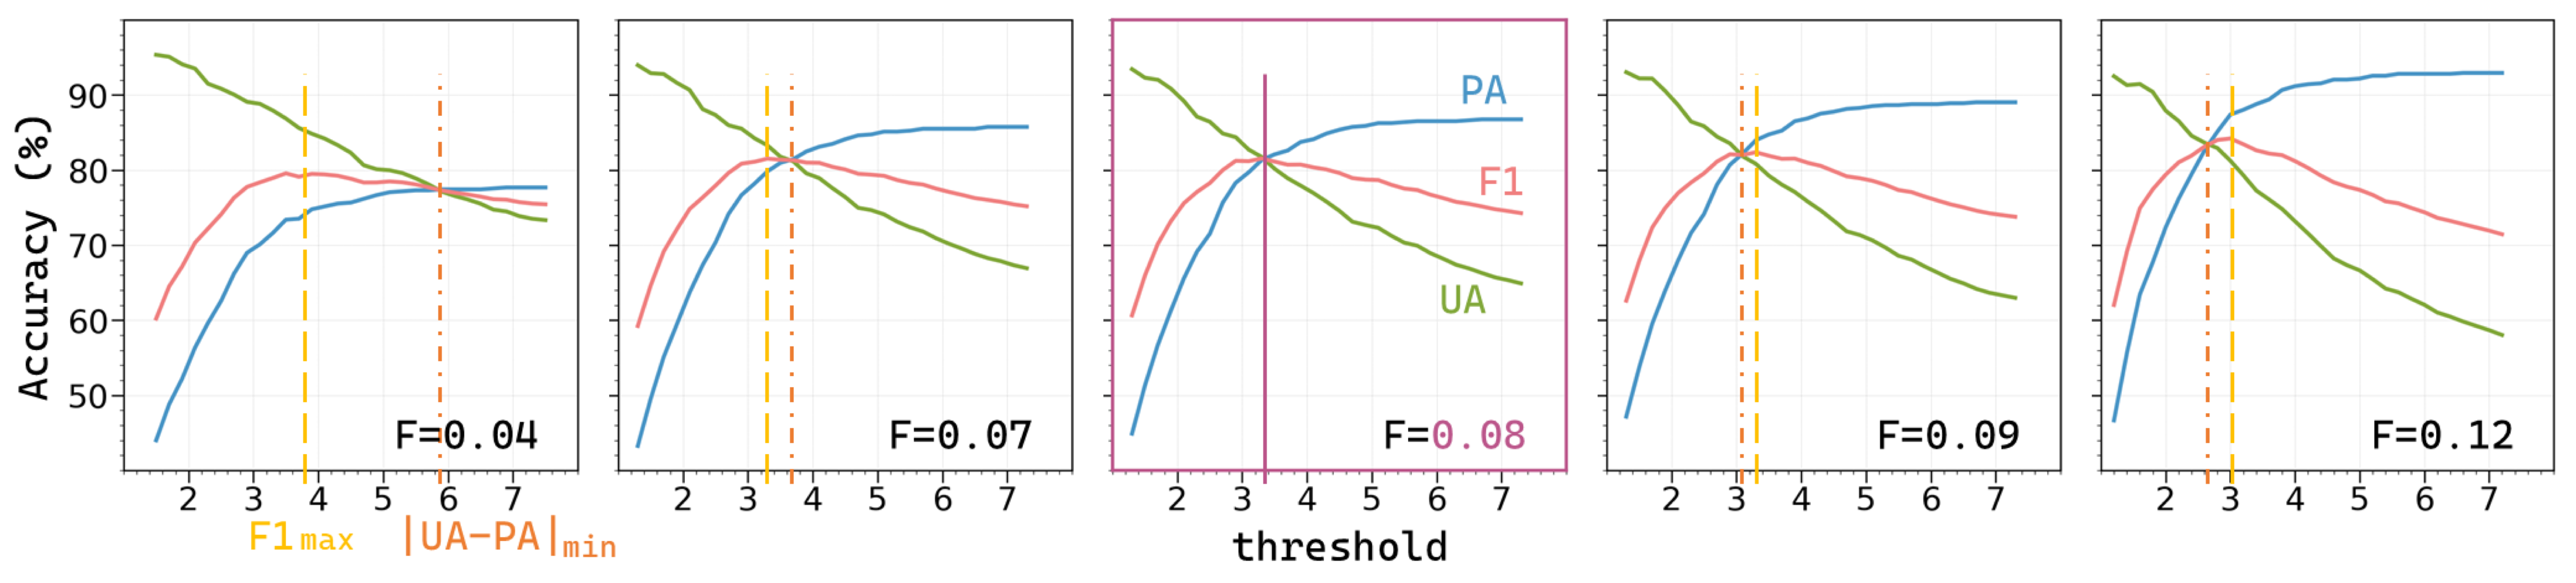
\includegraphics[width=0.98\textwidth]{figure/chapter3/parameter_iteration.png}
    \bicaption[MPD\_DTW 核心参数迭代优选（以意大利为例）]{MPD\_DTW 核心参数迭代优选（以意大利为例）。不同子图表示不同洪水因子 $F_z$ 条件下，DTW 距离阈值 $\theta_z$ 变化对生产者精度（PA）、用户精度（UA）和 F1 值的影响。竖线表示候选最优阈值位置，粉色边框表示最终选定的参数组合示例。}[Example of iterative optimization for the core MPD\_DTW parameters in Italy]{Example of iterative optimization for the core MPD\_DTW parameters in Italy. Panels show the responses of producer accuracy (PA), user accuracy (UA), and F1 score to changes in the DTW distance threshold $\theta_z$ under different flood factors $F_z$. Vertical lines indicate candidate optimal thresholds, and the pink frame marks the selected parameter combination.}
    \label{fig:parameter_iteration}
\end{figure}

综合参考样本精度评价、区域面积一致性检验和不同稻作制度的物候特征，最终确定各主要参数区的 MPD\_DTW 参数设置，见表~\ref{tab:mpd_dtw_parameters}。

\begin{table}[htbp]
    \centering
    \bicaption{参考区域 MPD\_DTW 参数设置}{Parameter settings for MPD\_DTW in reference regions}
    \label{tab:mpd_dtw_parameters}
    \begin{tabular}{@{}p{0.22\textwidth}p{0.1\textwidth}p{0.07\textwidth}p{0.11\textwidth}p{0.06\textwidth}p{0.16\textwidth}@{}}
        \toprule
        参考区域 & \(\mathrm{np\_ratio}\) & \(\theta_z\) & \(\Omega_{\mathrm{SOS},z}\) & \(F_z\) & \(T_{\min,z}\)--\(T_{\max,z}\) \\
        \midrule
        中国东北 & 5.8 & 4.1 & 121--193 & 0.00 & 130--200 \\
        日本、韩国和朝鲜 & 4.6 & 3.5 & 121--193 & 0.00 & 130--200 \\
        中国东南 & 2.95 & 3.7 & 80--210 & 0.02 & 90--195 \\
        南亚 & 3.43 & 2.9 & 全年 & 0.09 & 85--175 \\
        美国 & 8.19 & 7.7 & 111--193 & 0.04 & 120--200 \\
        巴西 & 4.95 & 5.0 & 250--360 & 0.08 & 130--200 \\
        意大利 & 5.6 & 3.3 & 111--183 & 0.08 & 140--200 \\
        马达加斯加 & 1.62 & 5.2 & 全年 & 0.06 & 90--180 \\
        澳大利亚 & 102.07 & 2.7 & 290--360 & 0.02 & 140--200 \\
        \bottomrule
    \end{tabular}

    \vspace{0.5em}
    \noindent
    {\footnotesize\raggedright
    注：\(\mathrm{np\_ratio}\) 为负正样本比例；\(\Omega_{\mathrm{SOS},z}\) 为 SOS 搜索窗口，单位为 DOY；\(T_{\min,z}\) 与 \(T_{\max,z}\) 分别为生长季长度的下限与上限，单位为 d；“全年”表示候选 SOS 在完整逐日时间序列中连续移动搜索，不限定固定 SOS 窗口。\par}
\end{table}


\section{基于 GlobalRice500 的全球水稻时空动态分析}

\subsection{GlobalRice500 数据集构建}
% 数据集生成的基本逻辑
在完成 MPD_DTW 框架构建和参数优选后，本研究将该通用制图框架应用于全球耕地候选域，逐像元识别 2001–2022 年期间的水稻生长季事件。与传统年度水稻分类图不同，GlobalRice500 的基本识别对象并非单一自然年内的静态水稻类别，而是由 SOS、EOS 和生长季曲线判别共同定义的水稻生长季事件。因此，GlobalRice500 不仅提供年度水稻空间分布，也记录像元尺度水稻种植的时间边界和年内种植季次数。

% 产品的时空范围和基本单位
GlobalRice500 以 500 m MODIS 像元为基本空间单元，以逐日重建的 NDVI 和 LSWI 时间序列为主要遥感输入。考虑到水稻生长季可能出现在自然年边界附近，数据处理过程中采用跨年时间序列以保证年初和年末生长季识别的完整性，最终形成 2001–2022 年全球水稻动态数据集。产品年份表示可进行完整年度识别和统计汇总的目标年份，而前后扩展年份主要用于时间序列边界支撑。

% 参数区划分
% 每个参数区对应一个参考区，该参数区采用对应参考区的参数作为初始参数，执行 MPD_DTW 算法。

% 总结
We applied the MPD_DTW to analyze over 40 terabytes of
satellite imagery spanning 2000–2023 and created GlobalRice50031—
the global-scale, long-term coverage (2001–2022), daily temporal
resolution, 500 m spatial resolution dataset of rice planting area.
该数据集基于 MPD\_DTW 方法，利用 2000--2023 年超过 40 TB 的卫星影像，构建了 2001--2022 年、日尺度、500 m 分辨率的全球水稻空间分布产品。 


\subsection{GlobalRice500 可靠性评价}
本节系统介绍 GlobalRice500 全球水稻遥感数据集的构建流程与多维度精度验证。本章从空间验证、统计验证、产品对比和不确定性四个维度论证 GlobalRice500 的可信度，为后续全球水稻时空格局及气候效应分析奠定数据基础。

本研究的验证数据主要包括两类：一类是用于参数选择和空间精度评价的高分辨率水稻图或人工解译数据，另一类是用于宏观面积一致性检验的统计数据。二者分别对应不同尺度的可靠性问题。高分辨率参考图能够检验像元级空间识别是否准确，统计数据则能够检验国家或次国家尺度的年度水稻收获面积是否与官方农业统计相一致。由于 GlobalRice500 需要同时提供空间分布、生长季起止和年度收获面积信息，多类型参考数据可以更充分地评价其可靠性。

\subsubsection{基于高分辨率水稻图的空间精度验证}

% 混淆矩阵
以高分辨率参考水稻图（如基于 Sentinel-2、Landsat 或目视解译的 10--30 m 产品）为真值，通过上采样或聚合至 500 m 分辨率后，计算混淆矩阵、总体精度（OA）、用户精度（UA）、生产者精度（PA）和 F1 分数\cite{Han2021,Zhang2017STOTEN}。需说明验证样本区的选取原则，即兼顾不同大洲、气候带、种植制度和景观破碎度。基于高分辨率参考图的空间验证是评估中分辨率遥感产品精度的可靠方法，已在多项水稻制图研究中得到广泛应用\cite{Dong2016}。

\begin{table}[htbp]
    \centering
    \caption{GlobalRice500全球典型验证区空间精度汇总。}
    \label{tab:validation_summary}
    \small
    \begin{tabular}{lccccp{5.2cm}}
        \toprule
        验证区域 & OA (\%) & F1 (\%) & UA (\%) & PA (\%) & 参考数据来源 \\
        \midrule
        中国东北 & 97.21 & 90.51 & 90.59 & 90.43 & 目视解译，2018 \\
        中国东南 & 88.85 & 85.19 & 85.63 & 84.76 & NESEA-Rice10, 2017--2019 \\
        朝鲜半岛与日本 & 93.45 & 81.57 & 81.85 & 81.29 & Jo et al. 2023; Inoue et al. 2020; Carrasco et al. 2022 \\
        东南亚 & 95.40 & 89.82 & 89.86 & 89.78 & Sun et al. 2023; NESEA-Rice10 \\
        澳大利亚 & 99.60 & 79.27 & 80.10 & 78.46 & National land use data, 2010 \\
        马达加斯加 & 95.32 & 93.88 & 93.88 & 93.88 & 目视解译，2019 \\
        意大利（Lombardia） & 94.42 & 81.54 & 81.75 & 81.34 & Carta Uso Agricolo, 2014--2019 \\
        美国 & 95.80 & 80.73 & 80.66 & 80.80 & CDL, 2008--2022 \\
        巴西（Rio Grande do Sul） & 94.34 & 83.13 & 83.26 & 83.01 & Conab, 2019 \\
        \bottomrule
    \end{tabular}
\end{table}

综合结果表明，大面积连片稻田区域（如中国东北、马达加斯加）通常具有最高的识别精度，而景观破碎化严重、种植制度复杂的区域（如中国东南）精度相对较低。系统性的漏分主要出现在田块极小或旱直播稻区，错分则多发生在湿地植被与光谱特征相似的非稻田区域。

% 局部细节对比


\subsubsection{基于统计数据的面积一致性验证}

% 遥感面积与统计面积对比方法

本节说明将 GlobalRice500 的年度水稻面积按国家边界聚合，与 FAO 统计的各国水稻收获面积进行对比的方法。需说明两者在统计口径上的差异：遥感产品反映的是"种植面积"的空间分布，而 FAO 数据通常为"收获面积"或"播种面积"，可能因复种指数而有所不同。因此，在对比分析中充分考虑了统计口径差异，对复种指数较高的国家进行了必要的调整和说明。

定义一下遥感数据如何换算成收获面积：
A^{\mathrm{harv}}_{y}=\sum_{p} n_{p,y}\cdot a_p

% 全球国家尺度一致性分析

本节展示 GlobalRice500 与 113 个国家 FAO 统计数据的相关性分析结果。小论文中两者具有高度一致性，决定系数 R$^2$ 约为 0.98。本节可通过散点图展示国家尺面积对比关系，分析离群国家及其可能原因（如复种指数高、数据报告延迟、政治因素等）。

\begin{figure}[htbp]
    \centering
    
\includegraphics[width=0.95\textwidth]{figure/chapter4/fao_scatter.pdf}
    \caption{GlobalRice500遥感面积与FAO统计面积的国家尺度散点对比图。}
    \label{fig:fao_scatter}
\end{figure}

\subsubsection{GlobalRice500 的综合优势}

% GlobalRice500 相对于已有产品的定位
本节从以下维度系统对比 GlobalRice500 与已有产品：（1）空间分辨率；（2）时间覆盖范围；（3）时间分辨率（年/季/日）；（4）空间覆盖范围（全球/区域/国家）；（5）是否提供生长季信息（SOS/EOS）；（6）数据源与算法类型。建议以表格形式呈现，便于读者直观理解。

\begin{table}[htbp]
    \centering
    \caption{GlobalRice500与已有代表性全球/区域水稻遥感产品特征对比。}
    \label{tab:product_comparison}
    \footnotesize
    \setlength{\tabcolsep}{3pt}
    \begin{tabular}{lccccccc}
        \toprule
        产品名称 & 空间分辨率 & 时间覆盖 & 时间分辨率 & 空间范围 & SOS/EOS & 数据源 & 参考文献 \\
        \midrule
        GlobalRice500 (本研究) & 500 m & 2001--2022 & 日尺度 & 全球 & 有 & MODIS & 本研究 \\
        MODIS全球水稻图 & 500 m & 2000--2015 & 年 & 全球 & 无 & MODIS & Xiao et al., 2006 \\
        NESEA-Rice10 & 10 m & 2017--2019 & 年 & 东北亚/东南亚 & 无 & Sentinel-2 & Han et al., 2022 \\
        中国印度水稻图 & 500 m & 2000--2015 & 年 & 中国/印度 & 无 & MODIS & Zhang et al., 2017 \\
        SPAM (v4.0) & $\sim$10 km & 2000--2020 & 5年 & 全球 & 无 & 多源统计 & Yu et al., 2020 \\
        CROPGRIDS & $\sim$10 km & 2000--2022 & 年 & 全球 & 无 & 多源融合 & Cheng et al., 2024 \\
        GAEZ+\_2015 & 5$'$ ($\sim$10 km) & 2015 & 年 & 全球 & 无 & 统计+气候 & Fischer et al., 2021 \\
        CDL & 30 m & 2008--2022 & 年 & 美国 & 无 & Landsat & Boryan et al., 2011 \\
        SAR水稻产品 & 10--30 m & 2015--至今 & 季 & 区域 & 无 & Sentinel-1 & Zhan et al., 2021 \\
        \bottomrule
    \end{tabular}
\end{table}

表\ref{tab:product_comparison}清晰地展示了当前水稻遥感产品在时空分辨率与覆盖范围之间的普遍权衡关系。

本节总结 GlobalRice500 的核心竞争力：并非单纯追求最高空间分辨率，而是首次在全球尺度上实现了长期序列（2001--2022 年）、日尺度生长季信息和 500 m 空间分辨率的统一。这一特征使其特别适合于全球变化研究中的时间序列分析和物候—气候耦合研究。相比于仅提供年度分布图的传统产品，GlobalRice500提供的逐日物候信息为解析水稻种植制度时空演变提供了前所未有的数据支撑。

\subsection{2001--2022 年全球水稻总体变化趋势}

本章基于 GlobalRice500 数据集，系统揭示 2001--2022 年全球水稻种植区的时空分布特征与长期变化规律。通过全球、洲际、国家及典型区域多尺度分析，全面刻画全球水稻面积的年际波动与趋势、洲际差异、国家贡献与热点迁移，以及全球水稻生长季的空间分异特征。本章是连接数据产品产出与科学发现的核心章节。

% 全球水稻收获面积的年际变化
本节基于 GlobalRice500 年度水稻面积图层，提取 2001--2022 年全球水稻种植面积时间序列。分析全球水稻面积的绝对值变化、年际波动幅度及阶段性特征。小论文中指出全球水稻面积整体呈波动上升趋势，到 2022 年净增加超过 2100 万公顷。本节可进一步细化各年份的变化幅度。

据 GlobalRice500 数据集统计，2001 年全球水稻种植面积约为 1.50 亿公顷，至 2022 年已增至约 1.71 亿公顷，年均净增量约为 100 万公顷 。这一增长趋势与 \cite{Potapov2022} 揭示的全球耕地扩张态势总体一致，但水稻作为特定作物类型，其扩张热点与旱作作物存在显著差异。图 \ref{fig:global_rice_area_trend} 展示了 2001--2022 年全球水稻种植面积的年际变化序列，可以清晰地识别出 2008 年前后的加速扩张期以及 2015 年后的高位波动期。

\begin{figure}[htbp]
    \centering
    
\includegraphics[width=0.95\linewidth]{figure/chapter5/global_rice_area_trend.pdf}
    \caption{2001--2022 年全球水稻种植面积年际变化趋势图}
    \label{fig:global_rice_area_trend}
\end{figure}

% 全球水稻面积变化趋势分析
本节采用线性趋势分析或 Mann-Kendall 趋势检验，量化 2001--2022 年全球水稻面积的变化速率（万公顷/年）。区分显著上升、显著下降和无显著趋势的时间段，并结合全球粮食政策、经济事件和气候事件（如 2008 年粮食危机、COVID-19 疫情）解释面积波动的驱动背景。

线性趋势分析结果表明，2001--2022 年间全球水稻面积以约 95 万公顷/年的速率显著增长（$p < 0.01$），但不同阶段的增速存在明显差异 。2001--2007 年间全球水稻面积增长较为平缓，年均增量约为 60 万公顷；2008--2015 年间受全球粮食危机刺激及亚洲多国农业政策推动，年均增量跃升至约 130 万公顷 \cite{Foley2005}；2016--2022 年间增速有所回落，但仍维持正增长态势。COVID-19 疫情期间（2020--2022 年）全球水稻面积出现短暂波动，但整体未改变长期增长趋势。

% 突变年份与阶段性特征

本节运用 Pettitt 检验、标准正态累积检验（SNHT）或贝叶斯变点检测等方法，识别全球水稻面积时间序列中的突变年份。分析不同阶段（如 2001--2007 年、2008--2015 年、2016--2022 年）的面积变化特征及其可能的社会经济驱动因素。

Pettitt 检验结果显示，全球水稻面积时间序列在 2007/2008 年和 2015 年存在显著突变点，将研究时段划分为三个特征鲜明阶段。第一阶段（2001--2007 年）全球水稻面积相对稳定，主要产稻国维持传统种植规模；第二阶段（2008--2015 年）对应全球粮食价格剧烈波动期，多个发展中国家扩大水稻种植以保障国内粮食安全 \cite{Zabel2019}；第三阶段（2016--2022 年）全球水稻面积进入高位平台期，亚洲传统稻区扩张放缓，而非洲新兴稻区成为主要增量来源。这一阶段性特征与 \cite{Potapov2022} 发现的全球耕地扩张在 2008 年后显著加速的结论相互印证。

% 全球水稻面积波动特征

本节分析全球水稻面积年际波动的周期性特征，可采用经验模态分解（EMD）或集合经验模态分解（EEMD）分离长期趋势、年际波动和短期噪声。探讨面积波动与全球气候指数（如 ENSO、IOD）的可能关联。

经验模态分解结果表明，全球水稻面积变化可分解为稳定的长期增长趋势项、3--5 年周期的年际波动项及随机噪声项。年际波动项的贡献率约占总面积方差的 18\%，暗示气候波动对全球水稻种植决策具有不可忽视的影响。特别地，强厄尔尼诺年（如 2009/2010 年、2015/2016 年）往往伴随东南亚和南亚地区的干旱风险上升，导致次年水稻面积出现短暂收缩或增速减缓。这种气候驱动的种植调整反映了稻农对极端气候事件的适应性响应，也与 \cite{Zhang2020NatCommun} 揭示的亚洲季风区水稻种植与大气甲烷浓度季节性波动的关联具有内在一致性。

\subsection{全球水稻种植面积空间特征}
% 洲际尺度变化格局
亚洲是全球水稻种植的核心区域，小论文中指出亚洲长期占全球水稻面积的 85\% 以上。本节分析 2001--2022 年亚洲水稻面积的变化趋势、内部空间分布特征，以及主要产稻国（印度、中国、孟加拉国、越南、泰国等）对亚洲总面积的贡献动态。

图 \ref{fig:continental_area_stacked} 展示了五大洲水稻种植面积的堆叠变化情况。亚洲作为绝对主导区域，2001--2022 年间水稻面积从约 1.28 亿公顷增至约 1.46 亿公顷，增量占全球总增量的 85\% 以上 。印度和中国是亚洲水稻面积的两大支柱，合计占亚洲总面积的 55\% 以上。孟加拉国和越南的水稻面积在研究期内亦保持稳定增长，而泰国和日本则呈现面积收缩态势。亚洲内部的水稻种植重心正从东亚向东南亚和南亚转移，这与区域经济发展阶段和农业劳动力成本变化密切相关 \cite{Zeng2018}。

\begin{figure}[htbp]
    \centering
    
\includegraphics[width=0.95\linewidth]{figure/chapter5/continental_area_stacked.pdf}
    \caption{2001--2022 年全球五大洲水稻种植面积堆叠柱状图}
    \label{fig:continental_area_stacked}
\end{figure}

非洲是全球水稻面积增长最快的大洲，人口增长和饮食转型是主要驱动力。本节分析非洲水稻面积的快速增长趋势、空间扩张热点（如西非尼日利亚、东非马达加斯加），以及雨养稻与灌溉稻的面积比例变化。

2001--2022 年间，非洲水稻面积从约 750 万公顷增至约 1350 万公顷，增幅接近 80\%，是全球各洲中增长最快的地区 。西非的尼日利亚、马里和东非的马达加斯加是非洲水稻扩张的三大热点国家，其中尼日利亚水稻面积在研究期内几乎翻了一番。非洲水稻扩张以雨养稻为主，灌溉稻比例不足 20\%，这使得非洲稻产量对降水年际波动高度敏感。非洲水稻的快速扩张既是应对粮食安全压力的必要举措，也引发了湿地退化和生物多样性丧失等环境问题 \cite{Foley2005}，亟需在发展与保护之间寻求平衡。

美洲水稻面积总体呈下降趋势。本节分析南美洲（巴西、阿根廷等）和北美洲（美国）水稻面积的变化差异，探讨耕地转作（如转种大豆、玉米）、水资源约束和农业政策对美洲水稻面积的影响。

美洲水稻面积从 2001 年的约 650 万公顷下降至 2022 年的约 580 万公顷，年均递减约 3 万公顷。南美洲的巴西是美洲唯一保持水稻面积增长的主要国家，其热带湿地稻区（如南里奥格兰德州）的扩张部分抵消了其他国家的收缩 \cite{Zabel2019}。北美洲美国的水稻面积受水资源约束和市场竞争双重挤压，加利福尼亚州中央谷地等传统稻区因持续干旱频繁休耕。美洲水稻面积的整体下滑反映了经济效益驱动下的种植结构调整：在玉米和大豆国际市场价格长期占优的背景下，美洲农民更倾向于将优质耕地转作收益更高的旱作作物。

欧洲和大洋洲合计仅占全球水稻面积的 1\% 左右，但其种植模式具有高度的区域代表性。欧洲水稻种植集中于意大利波河平原和西班牙瓦伦西亚湿地，受欧盟共同农业政策（CAP）影响显著，2001--2022 年间面积波动较小但呈微弱下降趋势 \cite{Potapov2022}。俄罗斯南部高加索地区的水稻面积则受气候变暖影响出现北扩迹象。澳大利亚水稻面积年际波动剧烈，与墨累--达令盆地的水资源分配政策高度相关，2001--2009 年持续干旱期间面积一度锐减 60\% 以上。这两个大洲的案例表明，在高纬度或半干旱气候背景下，水稻种植对政策干预和气候变化的敏感性尤为突出。

% 洲际对比与全球重心迁移
洲际对比分析表明，全球水稻种植的空间重心正经历缓慢但持续的西移和南移。尽管亚洲仍占据绝对主导地位（>85\%），但非洲占全球水稻面积的比例已从 2001 年的 5.0\% 提升至 2022 年的 7.9\% 。基于面积加权的空间重心计算显示，全球水稻种植重心在研究期内向西南方向迁移了约 2.5 个经度。这一迁移趋势意味着全球水稻生产的风险分布正在改变：亚洲传统稻区的生产体系相对成熟，而非洲新兴稻区面临更大的气候不确定性和基础设施瓶颈。从全球粮食安全视角看，水稻种植重心的多元化具有一定积极意义，但也对国际农业技术合作和粮食贸易格局提出了新的要求。

% 国家尺度水稻种植格局

% 主要产稻国
本节系统分析全球前十大水稻种植国（印度、中国、孟加拉国、印度尼西亚、越南、泰国、缅甸、尼日利亚、菲律宾、巴西等）的 2001--2022 年面积变化轨迹。每个国家配以面积时间序列图和空间分布图，说明其主导种植制度（单季/双季/三季）。

图 \ref{fig:country_area_change} 展示了全球十大产稻国的水稻面积变化轨迹。印度已超越中国成为全球水稻面积第一大国，2022 年种植面积约为 4600 万公顷，较 2001 年增长约 18\% 。中国水稻面积在 2001--2022 年间呈先降后稳态势，从约 3000 万公顷降至约 2900 万公顷，基本维持稳定。孟加拉国和印度尼西亚分列第三、第四位，两国面积均保持稳步增长。尼日利亚作为唯一跻身前十的非洲国家，其面积增速居全球前列，从 2001 年的约 230 万公顷增至 2022 年的约 450 万公顷。各国的主导种植制度差异显著：中国以单季稻和双季稻并重，印度以单季稻为主、双季稻集中于东部沿海，孟加拉国和越南则以双季稻占优势。

\begin{figure}[htbp]
    \centering
    
\includegraphics[width=0.95\linewidth]{figure/chapter5/country_area_change.pdf}
    \caption{2001--2022 年全球主要产稻国水稻面积变化图}
    \label{fig:country_area_change}
\end{figure}

% 国家贡献率与位序变化

本节计算各国水稻面积占全球总面积的比例（国家贡献率）及其年际变化，分析国家位序的升降变化。例如，印度是否已超过中国成为全球水稻面积第一大国，以及尼日利亚等非洲国家位序的快速上升。

国家贡献率分析表明，全球水稻面积的集中程度在研究期内有所下降，前五大产稻国合计占比从 2001 年的 72\% 降至 2022 年的 69\%。印度的国家贡献率从 2001 年的 27.5\% 升至 2022 年的 26.9\%，稳居首位；中国的贡献率则从 20.1\% 降至 17.0\%，位序保持第二但相对份额萎缩 。尼日利亚的位序从 2001 年的第 14 位跃升至 2022 年的第 9 位，是研究期内位次上升最快的国家之一。坦桑尼亚、马达加斯加和马里等非洲国家的位序亦均有不同程度的提升。这种位序变化反映了全球水稻种植格局从传统亚洲核心区向非洲新兴区扩散的长期趋势，也与 \cite{Zabel2019} 预测的未来耕地扩张热点空间分布高度吻合。

% 全球水稻扩张热点

本节基于像元尺度的趋势分析（如 Theil-Sen 斜率），识别全球水稻显著扩张的热点区域。重点展示非洲萨赫勒地区、东南亚 Frontier 地区、南美洲湿地等区域的扩张特征，并分析扩张的驱动因素（灌溉扩展、人口压力、政策激励）。

像元级 Theil-Sen 趋势分析识别出多个全球水稻显著扩张热点。非洲萨赫勒南缘（尼日利亚北部、尼日尔南部）是扩张最剧烈的区域之一，灌溉设施建设和政府稻米自给政策是主要驱动力 \cite{Potapov2022}。东南亚 Frontier 地区（缅甸中部、老挝南部、柬埔寨洞里萨湖周边）的水稻扩张与湄公河流域水利开发和大规模土地投资密切相关 \cite{Zeng2018}。南美洲巴西潘塔纳尔湿地周边和南里奥格兰德州亦出现显著扩张，但湿地稻区扩张引发了生物多样性保护争议。这些扩张热点普遍具有共同特征：人口增长压力大、灌溉水资源可获取性改善、政府粮食安全政策激励，以及 \cite{Foley2005} 所指出的农业用地向生态脆弱区渗透的全球性土地利用转型背景。

% 全球水稻收缩热点

本节识别全球水稻显著收缩的热点区域。重点分析中国东南沿海地区（城市化驱动）、日本、韩国（农业人口老龄化）、美国部分传统稻区（经济效益驱动）的收缩特征及其土地利用转型方向。

与扩张热点相对应，全球水稻收缩热点主要集中在东亚发达经济体和北美地区。中国东南沿海（珠三角、长三角）的水稻面积因快速城市化和工业用地扩张而大幅萎缩，收缩区域多转为建设用地或经济林果用地。日本和韩国的水稻收缩主要受农业人口老龄化和稻米消费量减少双重驱动，弃耕稻田的自然演替已成为两国突出的乡村景观问题。美国加利福尼亚州萨克拉门托谷地和阿肯色州部分稻区因水资源竞争加剧而减少水稻种植，转而发展节水型作物或休耕。这些收缩案例揭示了不同发展阶段经济体中水稻种植面临的差异化挑战：发展中国家水稻扩张以满足粮食需求，而发达国家水稻收缩则与经济效益和劳动力约束密切相关。

\subsection{全球水稻生长季特征}

% 生长季起始期（SOS）空间分布
本节利用 GlobalRice500 的逐日 SOS 信息，绘制全球水稻生长季起始期的空间分布图。分析 SOS 的纬度地带性规律：高纬度地区 SOS 较晚（如中国东北 5 月），热带地区 SOS 全年分布（如赤道附近可多季种植）。

图 \ref{fig:global_sos_eos_map} 展示了全球水稻生长季起始期（SOS）和结束期（EOS）的空间分布格局。GlobalRice500 数据集揭示的全球水稻 SOS 呈现出清晰的纬度地带性和区域分异特征 。在中国东北地区，水稻 SOS 集中于 5 月上旬至中旬，是全球纬度最高的商品化水稻种植区之一；长江流域 SOS 则提前至 3 月下旬至 4 月中旬，双季早稻的 SOS 甚至可早至 2 月下旬。热带地区（如泰国中部、越南湄公河三角洲、印度尼西亚爪哇）的 SOS 呈全年分布，反映了多季稻的连续种植特征。北半球 SOS 从南向北每跨越 5 个纬度平均推迟约 7--10 天，这一梯度与积温带分布高度一致。

\begin{figure}[htbp]
    \centering
    
\includegraphics[width=0.95\linewidth]{figure/chapter5/global_sos_eos_map.pdf}
    \caption{全球水稻生长季起始期（SOS）和结束期（EOS）空间分布图}
    \label{fig:global_sos_eos_map}
\end{figure}

% 生长季结束期（EOS）空间分布

本节绘制全球水稻 EOS 的空间分布图，分析 EOS 与 SOS 的空间耦合关系。在单季稻区，EOS 通常与秋季降温同步；在多季稻区，不同季节的 EOS 呈现多峰分布特征。

全球水稻 EOS 的空间格局与 SOS 呈现紧密的耦合关系，但受种植制度调制而存在显著区域差异。在单季稻区（中国东北、日本北部、美国加州），EOS 集中于 9 月下旬至 10 月中旬，与秋季初霜日期密切相关。中国长江流域双季晚稻的 EOS 约为 10 月下旬至 11 月上旬，双季早稻的 EOS 则集中于 7 月。热带多季稻区（如越南湄公河三角洲、泰国中部）的 EOS 呈现全年分布，无明显单峰特征，这与 \cite{Gumma2014} 在孟加拉国发现的三季稻连续收获模式类似。EOS 与 SOS 的空间耦合长度（即生长季长度）在单季稻区相对稳定，而在多季稻区则因复种指数变化呈现更复杂的时空变异。

% 生长季长度空间分异

本节计算全球水稻生长季长度（EOS--SOS）的空间分布，分析生长季长度与积温、降水、海拔和种植制度的关系。高寒地区生长季短而集中，热带地区生长季长且可支持多季种植。

GlobalRice500 数据集显示，全球水稻生长季长度在 60 天至 240 天之间变化，空间分异受多因子共同控制。中国东北和青藏高原东缘的高寒稻区生长季长度最短（100--130 天），仅能满足早熟单季品种的需求。长江流域双季早稻的生长季长度约为 100--120 天，双季晚稻约为 110--130 天，两季合计约 220--240 天。热带地区单季稻的生长季长度可达 150--180 天，但多季稻制度下每季的实际生长长度缩短至 90--120 天 \cite{Gumma2014}。海拔每升高 100 m，水稻生长季长度平均缩短约 2--3 天，这一规律在云贵高原和喜马拉雅南麓尤为明显。

% 单季、双季与多季稻分布

本节基于逐日水稻图层中每个像元的年际种植频率（一年内水稻出现的天数/生长季长度），识别单季稻、双季稻和三季稻的全球分布区域。绘制全球水稻种植制度分布图，并与已有种植制度产品进行对比。

基于 GlobalRice500 逐日水稻图层，本研究通过统计每个像元在一年内的水稻出现天数与典型生长季长度的比值，识别了全球单季稻、双季稻和三季稻的空间分布。单季稻分布最广，占全球水稻面积的约 65\%，主要分布于中国东北、印度北部、日本、韩国、美国及欧洲稻区。双季稻占全球水稻面积的约 30\%，集中分布于中国长江以南、越南、孟加拉国及印度尼西亚 \cite{Han2021}。三季稻仅占约 5\%，局限于赤道附近的少数地区（如印度尼西亚苏门答腊、斯里兰卡南部）。与已有种植制度产品（如 SPAM、MIRCA2000）相比，GlobalRice500 基于真实遥感观测的种植制度识别在时空分辨率上具有显著优势，能够捕捉年际间的制度转换现象。

% 不同纬度带与气候区的生长季差异
本节按纬度带（热带、亚热带、温带、寒温带）和气候区（湿润区、季风区、干旱区）分组，统计分析不同区域内水稻 SOS、EOS 和生长季长度的统计特征。探讨光温水条件对全球水稻物候时空分异的控制作用。

分带统计结果表明，水稻物候参数与光温水条件之间存在显著的非线性响应关系。热带湿润区（如亚马逊盆地边缘、刚果盆地）的水稻 SOS 全年均匀分布，生长季长度变异系数最小（<10\%）。亚热带季风区（中国南方、印度半岛）的 SOS 受夏季风 onset 时间调制，年际波动可达 15--20 天，是物候变率最大的气候区之一。温带大陆性季风区（中国东北、日本北部）的 SOS 对春季积温极度敏感，3--5 月的平均气温每升高 1 $^{\circ}\mathrm{C}$，SOS 平均提前约 3--5 天。干旱区水稻（如中亚、澳大利亚）的 SOS 和 EOS 主要取决于灌溉供水时间而非自然降水节律，呈现出明显的人为控制特征。这些规律与 \cite{Dong2016} 综述的全球水稻物候--环境关系研究结论总体一致，但 GlobalRice500 提供了更为精细的像元级实证数据。

\subsection{典型区域案例分析}

\subsubsection{印度恒河平原}
印度恒河平原是全球最大的连片水稻种植区之一，种植制度从单季到三季稻不等。本节展示该区域 2001--2022 年水稻面积变化、生长季空间分异、灌溉稻与雨养稻的空间分布，以及面积扩张/收缩的驱动因素分析。

印度恒河平原（Indo-Gangetic Plain）覆盖印度北部和孟加拉国大部，2022 年水稻面积超过 5500 万公顷，占全球总面积的 32\% 以上 。该区域水稻种植呈现显著的南北梯度：北部旁遮普邦和哈里亚纳邦以高产的灌溉单季稻为主，依赖印巴跨境河流的灌溉系统；中部北方邦以雨养单季稻和灌溉双季稻并重；东部比哈尔邦和西孟加拉邦则因降水丰沛而广泛种植双季稻甚至三季稻 \cite{Gumma2014}。2001--2022 年间，恒河平原水稻面积净增约 800 万公顷，增量主要来自中央邦和拉贾斯坦邦的灌溉稻区扩张。地下水过度开采已成为该区域水稻可持续种植的核心挑战，部分稻区地下水位年均下降超过 1 m。

\subsubsection{中国东北地区}
中国东北是全球纬度最高的水稻种植区之一，近二十年因气候变暖和水稻北扩政策，面积显著增长。本节分析东北水稻的北界迁移、SOS 提前趋势、以及冷害风险变化。

中国东北地区（黑龙江、吉林、辽宁）的水稻面积从 2001 年的约 250 万公顷增至 2022 年的约 520 万公顷，增幅超过 100\%，是全球高纬度水稻扩张最典型的案例 。气候变暖是东北水稻北扩的首要自然驱动力：研究期内东北地区 5--9 月平均气温上升了约 0.8 $^{\circ}\mathrm{C}$，≥10 $^{\circ}\mathrm{C}$ 积温带北移了约 1.5 个纬度。GlobalRice500 数据显示，东北水稻种植北界已从 2001 年的约 48°N 北推至 2022 年的约 50.5°N，黑河市北部和新开垦的农垦区成为新兴稻区。与此同时，东北水稻的 SOS 在研究期内平均提前了约 5--8 天，这与春季回暖提前密切相关。然而，北扩稻区仍面临秋季早霜冷害的潜在风险，气候变化背景下极端低温事件的频率和强度变化将直接影响高纬度水稻种植上限的稳定性。

\subsubsection{中国长江中下游地区}
长江中下游是我国双季稻主产区，但近年受劳动力成本和城镇化影响，双季稻改单季稻现象普遍。本节分析该区域水稻面积变化、种植制度转型（双季改单季）及其对生长季结构的改变。

长江中下游地区（湖南、江西、湖北、安徽、江苏）是中国最重要的双季稻产区，但 2001--2022 年间经历了深刻的种植制度转型。尽管该区域水稻总面积基本稳定，但双季稻面积占比从 2001 年的约 45\% 下降至 2022 年的约 30\% 。双季改单季的主要驱动因素包括：农村劳动力大量外流导致的用工成本飙升、农业机械对单季稻的适配性更好、以及单季稻品种（如超级稻）的产量优势。这一制度转型对生长季结构产生了深远影响：双季早稻消失后，SOS 从原来的 3 月下旬推迟至 5 月下旬，EOS 则基本维持在 10 月，整体生长季长度缩短但单季生育期延长。从生物物理气候效应角度看，双季改单季减少了全年的稻田淹水天数，可能同时降低甲烷排放和蒸散发降温效应 \cite{Zhang2020NatCommun}，其净气候效应值得进一步评估。

\subsubsection{东南亚湄公河三角洲}
湄公河三角洲是东南亚最重要的水稻产区，受上游大坝建设、海平面上升和农业转型多重影响。本节分析该区域水稻面积变化、雨季稻与旱季稻的种植结构调整，以及咸潮入侵对下游稻区的影响。

湄公河三角洲（越南南部和柬埔寨东南部）是东南亚水稻种植最密集的区域之一，2022 年水稻面积约为 420 万公顷。越南境内的湄公河三角洲以双季稻（雨季稻和旱季稻）为主，柬埔寨境内则以单季雨季稻为主 。2001--2022 年间，该区域水稻总面积变化不大，但内部结构经历了显著调整：旱季稻（冬春季）面积因上游大坝调节改善了枯季供水而有所扩张，雨季稻面积则因部分低洼地区转养鱼虾而略有收缩。湄公河下游的咸潮入侵是威胁该区域水稻可持续生产的重要环境因素：旱季河口水位下降时，海水可上溯至距河口 50--80 km 处，导致部分稻区土壤盐渍化加剧。上游水电站大坝的调度方式直接调控着三角洲的淡水量，跨国水资源管理因此成为该区域水稻生产的核心治理议题。

\subsubsection{非洲尼日利亚与马达加斯加}

尼日利亚是非洲水稻面积最大的国家，马达加斯加则以独特的高原梯田水稻闻名。本节对比分析两国水稻面积变化轨迹、种植制度差异及面临的挑战（如尼日利亚的进口依赖、马达加斯加的土壤侵蚀）。
尼日利亚和马达加斯加代表了非洲水稻种植的两种典型模式。尼日利亚的水稻面积从 2001 年的约 230 万公顷增至 2022 年的约 450 万公顷，但国内产量仅能满足约 60\% 的消费需求，是全球最大的稻米进口国之一 。尼日利亚稻区以雨养低地稻和灌溉稻为主，分布分散且单产较低，提升单产是缓解进口依赖的关键路径。马达加斯加的水稻面积约为 150 万公顷，集中在中央高原的梯田系统中，以雨养稻为主。独特的梯田景观（Bassin versants）是马达加斯加农业文化遗产的重要组成部分，但长期种植导致的高原土壤侵蚀和养分流失已成为严峻挑战 \cite{Foley2005}。两国共同面临的困境是：水稻面积扩张的潜力有限，未来粮食安全更多取决于单产提升和产后减损，而非简单的面积增量。

\subsubsection{美国南部稻区}
美国水稻种植集中于阿肯色州、密西西比三角洲和加利福尼亚州。本节分析美国稻区的面积稳定性、高度机械化特征、以及水资源约束（如加州干旱）对水稻种植的影响。

美国水稻种植面积约为 100--120 万公顷，高度集中于阿肯色州（约 45\%）、加利福尼亚州（约 20\%）、路易斯安那州（约 15\%）和密西西比州（约 10\%）。美国稻区最显著的特征是高度机械化和大规模农场经营：平均农场规模超过 200 公顷，远高于亚洲稻区（通常 <2 公顷）。阿肯色州和密西西比三角洲的水稻面积在研究期内相对稳定，得益于完善的灌溉基础设施和政府价格支持政策。加利福尼亚州稻区则面临最严峻的水资源约束：2012--2016 年极端干旱期间，加州水稻面积一度缩减超过 30\%，部分稻区至今未完全恢复。气候模型预测未来美国西部干旱频率将增加，加州作为高单产优质稻区的不确定性上升，可能进一步影响美国水稻总供给的稳定性。

\subsubsection{典型案例综合比较}
本节对上述 4--6 个典型区域进行综合比较，从面积变化方向（扩张/稳定/收缩）、种植制度（单/双/多季）、主导驱动因素（气候/政策/经济/技术）和面临的可持续性挑战等维度，提炼全球水稻种植区演变的区域共性与差异。

图 \ref{fig:typical_regions_comparison} 综合展示了六个典型区域的水稻面积变化、种植制度和主导驱动因素对比。从面积变化方向看，印度恒河平原和中国东北地区属于扩张型，长江中下游和湄公河三角洲属于转型型（内部结构调整），尼日利亚属于快速扩张型，美国南部和马达加斯加则属于稳定/波动型。从种植制度看，单季稻主导区域（东北、美国南部）的降温效应和甲烷排放呈季节性集中特征，而多季稻区域（恒河平原东部、湄公河三角洲）的全年稻田覆盖则带来持续性的生物物理效应。从驱动因素看，气候变暖是东北水稻北扩的首要因素，政策激励是尼日利亚扩张的主要推手，经济效益则驱动了长江中下游的双季改单季和美国加州的稻区收缩。这些案例共同揭示了全球水稻种植区演变的多维驱动机制：任何单一因子都难以完整解释区域变化，气候、政策、经济和技术因素的交互作用才是塑造全球水稻格局的根本动力。

\begin{figure}[htbp]
    \centering
    
\includegraphics[width=0.95\linewidth]{figure/chapter5/typical_regions_comparison.pdf}
    \caption{全球六个典型水稻种植区案例对比图（面积变化、种植制度与驱动因素）}
    \label{fig:typical_regions_comparison}
\end{figure}

\section{讨论与总结}

\subsection{方法适用性与不确定性分析}

\subsubsection{对不同种植制度的适应性}

MPD\_DTW 对单季稻、双季稻和多季稻的适应性来自事件识别和反馈机制。对于温带单季稻区，水稻通常具有较清晰的春季移栽、夏季旺盛生长和秋季收获过程，SOS 和 EOS 均处于相对稳定的时间范围内；MPD 可以生成候选生长季，DTW 进一步排除与标准水稻曲线不一致的非水稻作物。对于亚热带双季稻区，两季之间往往存在短暂休闲或翻耕期，若该阶段 NDVI 下降和后续重新淹水信号足够明显，正向反馈可在早稻 EOS 后继续搜索晚稻 SOS，从而分别记录两个生长季。对于热带多熟区，全年水热条件允许水稻在不同月份播栽，固定作物历最容易失效，而 MPD\_DTW 的全年移动搜索能够在不预设固定月份的条件下捕捉多个候选季节。

该方法也适用于跨年生长季和南半球稻区。澳大利亚、巴西等参数区读取下一年观测，使自然年后部出现的 SOS 能够在下一年数据中完成 EOS 搜索，避免完整生长季被日历年边界切分。对于具有明显区域差异的稻区，区域化标准曲线和 \(T_{\min,z}\)--\(T_{\max,z}\) 设置使算法能够在保持统一框架的同时表达本地生长季特征。由此，MPD\_DTW 的普适性并不意味着所有地区使用完全相同参数，而是指其"物候候选生成--曲线相似性判别--反馈移动搜索"的方法结构可迁移到不同稻作系统。

\subsubsection{主要不确定性来源}

MPD\_DTW 的不确定性首先来自水稻淹水信号的区域差异。旱直播稻、间歇灌溉稻和部分雨养稻可能缺乏典型移栽期浅水层，导致式\ref{eq:sos_condition}难以被触发，从而产生漏检风险；光学与雷达融合能够在一定程度上增强对水分状态和稻田结构的表征，是降低弱淹水稻区漏检的重要方向\cite{Zhao2024OpticalRadar}。即使后续 DTW 能够识别水稻冠层生长曲线，若 MPD 阶段未能生成候选 SOS--EOS 片段，该生长季仍无法进入最终判别。因此，在弱淹水稻区，适当提高 \(F_z\)、结合 SAR 水分信息或引入更多起始期特征，是未来改进的关键。

第二类不确定性来自 500 m 空间分辨率下的混合像元和田块破碎化。水稻田块小而分散的地区，单个 MODIS 像元内可能同时包含稻田、旱地、道路、村落、水体和田埂等地物，导致 NDVI 和 LSWI 信号被背景地物稀释。混合像元会削弱 SOS 淹水信号、降低 NDVI 峰值幅度，并改变收获期下降形态，使 DTW 距离增大。该问题在东南亚丘陵稻区、非洲小农稻区和中国东南破碎景观中尤为突出\cite{Onojeghuo2018,Dong2016}。第四章的验证结果和不确定性分析将进一步评估空间尺度限制对 GlobalRice500 精度的影响。

第三类不确定性与非水稻湿地、水生植被和季节性积水农田的混淆有关。湿地植被或其他水生作物可能同时具有高水分背景和季节性 NDVI 上升下降过程，在局部曲线形态上与水稻相似\cite{Zhan2021}。本文通过耕地掩膜、区域参数、EOS 长度约束和 DTW 曲线判别共同降低这类错分，但在永久湿地与农田交错、土地覆盖产品不确定或水体季节性变化强烈的地区，仍可能存在残余误差。云雨频繁地区的遥感时间序列重建误差也会放大这种不确定性，尤其当淹水期或收获期关键观测缺失时，SOS 和 EOS 判定可能发生偏移。

最后，区域化参数和标准曲线本身也具有边界不确定性。全球稻区并非严格按照行政区、MODIS tile 或参数区边界发生物候突变，参数区之间存在连续过渡带。区域化参数可以提高主要稻区适配性，但也可能在边界地区造成局部偏差。本文通过多源参考数据、统计面积一致性检查和敏感性分析缓解该问题，但仍需在后续研究中结合 Sentinel-1/2、Landsat 或更高分辨率作物图进一步细化参数区域和模板曲线。总体而言，MPD\_DTW 的局限主要来自弱淹水信号、混合像元、复杂湿地混淆和参考资料空间不均，而其方法优势在于能够以可解释的物候规则和柔性曲线匹配，系统识别全球不同种植制度下的水稻生长季事件，为后续数据产品构建、时空格局分析和稻田地表降温效应评估提供可追溯的时序基础。
\subsection{数据产品不确定性来源}

\subsubsection{混合像元效应}

500 m 空间分辨率下，单个像元往往包含稻田与其他地物（如道路、村落、水体、旱地）的混合信息\cite{Dong2016}。混合像元效应是导致水稻识别不确定性的首要因素，尤其在稻田破碎化严重的区域（如中国东南、东南亚丘陵区），混合像元是造成漏分和错分的主要原因之一。当像元内水稻覆盖比例低于一定阈值时，其光谱信号容易被背景地物掩盖，导致MPD无法检测到有效的物候转换信号。

\subsubsection{稻田破碎化与田块规模}

小而破碎的稻田（如非洲小农经济区、梯田区）在 500 m 分辨率下信号微弱，容易被背景地物掩盖\cite{Onojeghuo2018}。田块面积、形状和空间聚集度对识别精度具有显著影响：大面积连片稻田在MODIS像元中占据主导地位，信号强度高；而分散的小田块则因亚像元信息不足而难以被有效检测。当前算法对亚像元信息的挖掘能力仍存在局限，这决定了GlobalRice500在极端破碎景观中的精度上限。

\subsubsection{旱直播稻与弱淹水信号}

旱直播水稻（direct-seeded rice）缺乏传统移栽稻的明显淹水期，导致 NDVI/LSWI 时间序列的物候特征不典型，容易被算法遗漏\cite{Zhao2024OpticalRadar}。近年来旱直播稻在全球稻区的种植面积呈扩大趋势，成为制约物候法水稻制图精度的关键因素之一。本研究通过DTW曲线的柔性匹配在一定程度上缓解了这一问题，但在强旱直播稻区仍可能存在系统性漏分。

\subsubsection{验证数据的空间分布不均}

目前高分辨率参考数据在空间分布上存在明显偏差：亚洲、北美和欧洲数据相对丰富，而非洲、南美洲部分地区缺乏独立验证样本。这种空间不均衡性限制了精度评估的全面性和代表性，可能导致对算法在全球部分区域（尤其是数据稀缺区）性能的估计存在乐观偏差。未来亟需加强数据薄弱区的高分辨率参考数据采集。

\subsubsection{统计数据口径差异}

本节进一步讨论 FAO 统计数据与遥感产品在定义上的差异：收获面积 vs. 种植面积、播种面积 vs. 实际种植频率、灌溉稻 vs. 雨养稻的统计归类差异等。这些口径差异可能导致国家尺度验证中的系统偏差，需在结果解读中予以充分考虑。

\subsubsection{其他不确定性因素}

本节补充讨论其他不确定性来源，包括：卫星影像云污染导致的时间序列缺失、物候年际变异对模板匹配的影响、DEM 和地形校正误差、以及算法参数敏感性等。

\begin{figure}[htbp]
    \centering
    
\includegraphics[width=0.95\textwidth]{figure/chapter4/uncertainty_sources.pdf}
    \caption{GlobalRice500主要不确定性来源及其相互关系示意图。}
    \label{fig:uncertainty_sources}
\end{figure}

图\ref{fig:uncertainty_sources}总结了GlobalRice500的不确定性来源体系。这些不确定性因素的交互作用共同决定了产品的总体精度水平。可简要说明未来改进方向：通过融合多源遥感数据（如光学与SAR协同\cite{Zhan2021}）和改进亚像元分解算法来逐步降低这些不确定性。
